\documentclass{article}

\usepackage[utf8]{inputenc}

\usepackage[T1]{fontenc}
\usepackage{lmodern}
\usepackage{amssymb}
%\usepackage{graphicx}
\usepackage{prooftree,amsmath,wasysym,xcolor,xspace}
\ifx\pdftexversion\undefined
\usepackage[dvips]{graphicx}
\else
\usepackage{graphicx}
\DeclareGraphicsRule{*}{mps}{*}{}
\fi
\usepackage{mathptmx}
\usepackage{stmaryrd}
\usepackage{eurosym}
\usepackage{amsbsy}
\usepackage{latexsym}
\usepackage{url}
\usepackage{suffix}
\usepackage{listings}
\usepackage{color}
\usepackage{verbatim}
\usepackage{citesort}
\usepackage{tikz}
\usepackage{pslatex}
\usepackage{comment}
\usepackage{times}
%\usepackage{space}
\usepackage{etex}
\usepackage{epstopdf}
%\usepackage{microtype}  % Looks better but may take more space (only works for pdflatex)
\usepackage[all]{xypic}

\newcommand{\upd}{\mathit{update}}
\newcommand{\pn}{\p}
\newcommand{\rtsyntax}[1]{\colorbox{lightgray}{\ensuremath{#1}}}
\newcommand{\ptilde}[1]{{\ensuremath{#1}}}
%\newcommand{\kf}[1]{\textsf{\upshape\small #1}\xspace}
\newcommand{\kf}[1]{\textup{\textsf{#1}}\xspace}
\newcommand{\constf}[1]{\textup{\textsf{#1}}}
\newcommand{\srsimple}[3]{\ensuremath{\bar{#1}[#2](#3)}}
\newcommand{\sr}[4]{\ensuremath{\srsimple{#1}{#2}{#3}.#4}}
\newcommand{\uu}{\ensuremath{u}}
\newcommand{\Ia}{\ensuremath{a}}
\newcommand{\Ic}{\ensuremath{c}}
\newcommand{\Iu}{\ensuremath{u}}
\newcommand{\Ik}{\ensuremath{k}}
\newcommand{\Ias}{\ensuremath{\alpha}}
\newcommand{\Ib}{\ensuremath{b}}
\newcommand{\y}{\ensuremath{y}}
\newcommand{\PP}{\ensuremath{P}}
\newcommand{\Q}{\ensuremath{Q}}
\newcommand{\R}{\ensuremath{R}}
\newcommand{\DD}{\ensuremath{D}}
\newcommand{\sasimple}[3]{\ensuremath{#1[#2](#3)}}
\newcommand{\sa}[4]{\ensuremath{\sasimple{#1}{#2}{#3}.#4}}
\newcommand{\pp}{\ensuremath{\at{\p}}}
\newcommand{\si}[2]{\ensuremath{#1[#2]}}
\newcommand{\sI}[1]{\ensuremath{\s_{#1}}}
%\newcommand{\sI}[1]{\ensuremath{\s^#1}}   vecchia versione
\newcommand{\sii}{\si{\s}{\p}}
\newcommand{\sij}{\si{\s}{\p_j}}
\newcommand{\siq}{\si{\s}{\q}}
\newcommand{\siip}{\si{\s'}{\p'}}
\newcommand{\sipp}{\si{\s'}{\p}}
\newcommand{\cc}{\ensuremath{c}}
\newcommand{\pset}{\ensuremath{\Pi}}
\newcommand{\inpset}[2][\Pi]{\ensuremath{\p_#2 \in #1}}
\newcommand{\kinpset}{\inpset{k}}
%\newcommand{\pset}{\ensuremath{\set{\participant{\p}_k}_{k\in K}}}
\newcommand{\out}[4]{\ensuremath{#1!\langle \pset,#2\rangle;#4}}
%\newcommand{\out}[4]{\ensuremath{#1!\langle \set{#3_k}_{k\in K},#2\rangle;#4}}
\newcommand{\outp}[3]{\ensuremath{#1!\langle \pset,#2\rangle}}
\newcommand{\outs}[4]{\ensuremath{#1!\langle #3,#2\rangle;#4}}
\newcommand{\e}{\ensuremath{e}}
\newcommand{\inp}[4]{\ensuremath{#1?( #3,#2);#4}}
\newcommand{\inpp}[3]{\ensuremath{#1?( #3,#2)}}
\newcommand{\inps}[4]{\ensuremath{#1?( #3,#2);#4}}
\newcommand{\x}{\ensuremath{x}}
\newcommand{\participant}[1]{\ensuremath{\mathtt{#1}}}
\newcommand{\q}{\ensuremath{\participant{q}}}
\newcommand{\p}{\ensuremath{\participant{p}}}
\newcommand{\sd}[4]{\ensuremath{#1!\langle\! \langle#3,#2\rangle \!\rangle;#4}}
\newcommand{\sdt}[4]{\ensuremath{#1^\top!\langle\! \langle#3,#2\rangle \!\rangle;#4}}
\newcommand{\sdp}[4]{\ensuremath{#1!^{\lev'}\langle\! \langle#3,#2\rangle \!\rangle.#4}}
\newcommand{\rd}[4]{\ensuremath{#1?(\!(#3,#2)\!);#4}}
\newcommand{\rdt}[4]{\ensuremath{#1^\top?(\!(#3,#2)\!).#4}}
\newcommand{\z}{\ensuremath{z}}
\newcommand{\pc}{\Par}
\newcommand{\s}{\ensuremath{s}}
\newcommand{\X}{\ensuremath{X}}
\newcommand{\defX}{\ensuremath{\kf{def} \ \Ddef\ \kf{in}\ }}
\newcommand{\Xsignature}{\ensuremath{\X(\at{x}, \at{y})}}
\newcommand{\Ddef}{\ensuremath{\Xsignature=\PP}}
\newcommand{\Ddefp}{\ensuremath{\Xsignature=\PP'}}
\newcommand{\defIn}[1]{\ensuremath{\kf{def} \ #1 \ \kf{in}\ }}
\newcommand{\defD}{\ensuremath{\kf{def}\ \DD \ \kf{in}\ }}
\newcommand{\DdefD}{\ensuremath{\kf{def}\ \Ddef \ \kf{in}\ }}
\newcommand{\defDp}{\ensuremath{\kf{def}\ \DD' \ \kf{in}\ }}
\newcommand{\proccall}[3]{\ensuremath{#1\langle\ptilde{#2},\ptilde{#3}\rangle}}
\newcommand{\proccallw}[3]{\ensuremath{#1\langle\ptilde{#2},\ptilde{#3}\rangle}}
\newcommand{\proccalldots}[3]{\ensuremath{#1\langle\ptilde{#2},\ptilde{#3}\rangle}}

\newcommand{\indexed}[4]{\ensuremath{\{#1_#3 : #2_#3\}_{#3 \in #4}}}

\newcommand{\values}{\ensuremath{\at{v}}}
\newcommand{\trival}[3]{\ensuremath{(#3,#2, #1)}}
\newcommand{\labval}[2]{\ensuremath{(#1, #2)}}
\newcommand{\anglep}[2]{\ensuremath{\langle #1, #2\rangle}}
\newcommand{\valheap}[3]{\ensuremath{( #3,\pset,#1 )}}
\newcommand{\valheaps}[3]{\ensuremath{( #3,#2,#1 )}}
\newcommand{\valheapj}[2]{\ensuremath{( #2,\{j\},#1 )}}
\newcommand{\valheapp}[2]{\ensuremath{( #2,\{\p\},#1 )}}
\newcommand{\valheapLess}[3]{\ensuremath{( #3,\pset\setminus \p,#1 )}}
\newcommand{\delheap}[3]{\ensuremath{(#3,{#2},#1 )}}
\newcommand{\labheap}[3]{\ensuremath{( #3,\pset,#1 )}}
\newcommand{\labheaps}[3]{\ensuremath{( #3,#2,#1 )}}
\newcommand{\labheapj}[2]{\ensuremath{( #2,\{j\},#1 )}}
\newcommand{\labheapp}[2]{\ensuremath{( #2,\{\p\},#1 )}}
\newcommand{\lsel}[4]{\ensuremath{#1 \oplus \anglep{\pset}{#2};#4}}
\newcommand{\lbranch}[2]{\ensuremath{#1 \&
({#2},\indexed{l}{\PP}{i}{I})}}
\newcommand{\lbranchi}[2]{\ensuremath{#1 \&
({#2},\indexed{l}{\PP}{i}{I})}}
\newcommand{\ifthenelse}[3]{\ensuremath{\kf{if}\ #1\ \kf{then}\ #2\ \kf{else}\ #3}}
\newcommand{\ift}[2]{\ensuremath{\kf{if}\ #1\ \kf{then}\ #2}}
\newcommand{\inact}{\ensuremath{\mathbf{0}}}
\newcommand{\nuc}[2]{\ensuremath{(\nu #1)#2}}
\newcommand{\AND}[2]{\ensuremath{#1\ \kf{and}\ #2}}
\newcommand{\NOT}[1]{\ensuremath{\kf{not}\ #1}}
\newcommand{\true}{\kf{true}}
\newcommand{\false}{\kf{false}}
\newcommand{\h}{\ensuremath{h}}
\newcommand{\mg}{\ensuremath{m}}
\newcommand{\va}{\ensuremath{v}}
\newcommand{\at}[1]{\ensuremath{\ptilde{#1}}}
\newcommand{\atw}[1]{\ensuremath{\ptilde{#1}}}
\newcommand{\Co}[1]{\ensuremath{C[#1]}}
\newcommand{\Par}{\ensuremath{\ |\ }}
\newcommand{\cas}{\ensuremath{r}}
\newcommand{\eq}{\ensuremath{$\diameter$}}

%SEMANTICA
\newcommand{\redsym}{\ensuremath{\longrightarrow}}
\newcommand{\red}[2]{\ensuremath{#1\redsym#2}}
\newcommand{\redM}[2]{\ensuremath{#1\redsym^*#2}}
\newcommand{\set}[1]{\ensuremath{\{#1\}}}
\newcommand{\sub}[2]{\ensuremath{\{#1/#2\}}}
\newcommand{\ssub}[2]{\ensuremath{\{#1/#2\}}}
\newcommand{\subO}[2]{\ensuremath{\set{\!\{#1/#2\}\!}}}

\newcommand{\sep}{\ensuremath{~\mathbf{|}~ }}

\newcommand{\Implies}{\ensuremath{\quad \Rightarrow \quad }}

\newcommand{\mqueue}[2]{\ensuremath{#1 : #2}}
\newcommand{\emptyqueue}[1]{\mqueue{\s}{\emptyset}}
\newcommand{\queue}{\ensuremath{\h}}
\newcommand{\stdqueue}{\mqueue{\s}{\queue}}
\newcommand{\qcomp}[2]{\ensuremath{#1 \cdot #2}}
\newcommand{\qtail}[1]{\ensuremath{\qcomp{\queue}{#1}}}
\newcommand{\qhead}[1]{\ensuremath{\qcomp{#1}{\queue}}}

\newcommand{\qappend}[1]{\mqueue{\s}{\qtail{#1}}}
\newcommand{\qpop}[1]{\mqueue{\s}{\qhead{#1}}}

\newcommand{\subst}[2]{\ensuremath{\{#1 / #2\}}}
\newcommand{\remove}[2]{\ensuremath{#1 \backslash \{#2\}}}

\newcommand{\freen}[1]{\ensuremath{\text{fn}(#1)}}
\newcommand{\dpv}[1]{\ensuremath{\text{dpv}(#1)}}
\newcommand{\fpv}[1]{\ensuremath{\text{fpv}(#1)}}
\newcommand{\rrule}[1]{[\text{#1}]}

%TIPI
\newcommand{\G}{\ensuremath{G}}
\newcommand{\Gv}[4]{\ensuremath{#1\to\pset:\langle#3\rangle.#4}}
\newcommand{\Gvr}[4]{\ensuremath{#1\to#2:\langle#3\rangle.#4}}
\newcommand{\U}{\ensuremath{U}}
\newcommand{\sid}[1]{\ensuremath{\textup{pn}(#1)}}
\newcommand{\pro}[2]{\ensuremath{#1\upharpoonright#2}}
\newcommand{\Ga}{\ensuremath{\Gamma}}
\newcommand{\D}{\ensuremath{\Delta}}
%\newcommand{\Dp}{\ensuremath{\D'}}
\newcommand{\T}{\ensuremath{T}}
\newcommand{\TQ}{\ensuremath{{\tt{T}}}}
\newcommand{\TG}{\ensuremath{{\mathsf{T}}}}
\newcommand{\Tp}{\ensuremath{T'}}
\newcommand{\ST}{\ensuremath{S}}
\newcommand{\TT}{\atw{\T}}
\newcommand{\SST}{\atw{S}}
\newcommand{\UT}{\ensuremath{U}}
\newcommand{\oT}[2]{\ensuremath{\;!\langle #2,#1\rangle}}
\newcommand{\iT}[2]{\ensuremath{?( #2,#1 )}}
\newcommand{\oTG}[2]{\ensuremath{\;\natural\langle #2,#1\rangle}}
\newcommand{\oTGp}[2]{\ensuremath{\;\natural'\langle #2,#1\rangle}}
\newcommand{\an}[1]{\ensuremath{\langle #1\rangle}}
\newcommand{\de}[3]{\ensuremath{#1\vdash#2:#3}}
\newcommand{\der}[3]{\ensuremath{#1\vdash#2\triangleright#3}}
\newcommand{\dom}[1]{\ensuremath{dom( #1)}}
\newcommand{\range}[1]{\ensuremath{range( #1)}}
\newcommand{\ty}{\textbf{t}}
\newcommand{\End}{\kf{end}}
\newcommand{\Bool}{\kf{bool}}
\newcommand{\Nat}{\kf{nat}}
%\newcommand{\setk}[1]{\ensuremath{\set{#1_k}_{k\in K}}}

\newcommand{\SelType}[2]{\ensuremath{\oplus(#1,#2)}}

\newcommand{\seltype}{\ensuremath{\oplus \langle \pset,\{l_i:\T_i\}_{i\in
I} \rangle }}
\newcommand{\seltypeG}{\ensuremath{\oplus(\pset,\{l_i:\pro{\G_i}\q\}_{i\in I})}}
\newcommand{\seltypeT}{\ensuremath{\oplus\{l_i:\pro{\T_i}\q\}_{i\in I}}}
\newcommand{\seltypeTp}{\ensuremath{\oplus\{l_i:\T_i\}_{i\in I}}}
\newcommand{\seltypeq}{\ensuremath{\oplus\langle\pset,l\rangle;\T}}
\newcommand{\seltypeqg}{\ensuremath{\oplus\langle\pset,l\rangle;\TG}}
\newcommand{\seltypeqj}{\ensuremath{\oplus\langle\{j\},l\rangle;\T}}
\newcommand{\seltypeqq}{\ensuremath{\oplus\langle\{\q\},l\rangle;\T}}
\newcommand{\seltypep}{\ensuremath{\oplus(\pset,l);\T'}}
\newcommand{\seltypezp}{\ensuremath{\oplus(\pset,l:\T_0;\T')}}
\newcommand{\seltypez}{\ensuremath{\oplus(\pset,l:\T_0)}}
\newcommand{\seltypei}{\ensuremath{\oplus\langle\pset,l_i\rangle;\T_i}}
\newcommand{\seltypej}{\ensuremath{\oplus(\pset,l_j);\T_j}}
\newcommand{\seltypesi}{\ensuremath{\oplus(\pset,l_{i})}}
\newcommand{\seltypesip}{\ensuremath{\oplus(\pset,l_{i'})}}
\newcommand{\seltypesipz}{\ensuremath{\oplus(\pset,l_{i_0})}}
\newcommand{\seltypesipzs}{\ensuremath{\oplus(\set\p,l_{i_0})}}
\newcommand{\seltypesipjz}{\ensuremath{\oplus(\pset\setminus \p,l_{i_0})}}
\newcommand{\seltypesipj}{\ensuremath{\oplus(\pset\setminus \p,l_{i'})}}
\newcommand{\seltypes}{\ensuremath{\oplus\langle\pset,l\rangle}}
\newcommand{\seltypesem}{\ensuremath{\oplus(\emptyset,l)}}
\newcommand{\seltypesemZ}{\ensuremath{\oplus(\emptyset,Z)}}
\newcommand{\branchtype}{\ensuremath{\&(\p,\{l_i:\T_i\}_{i\in I})}}
\newcommand{\branchtypeq}{\ensuremath{\&(\q,\{l_i:\T_i\}_{i\in I})}}
\newcommand{\branchtypeG}{\ensuremath{\&(\p,\{l_i:\pro{\G_i}\q\}_{i\in I})}}
\newcommand{\branchtypeT}{\ensuremath{\&\{l_i:\pro{\T_i}\q\}_{i\in I}}}
\newcommand{\branchtypeTp}{\ensuremath{\&\{l_i:\T'_i\}_{i\in I}}}
\newcommand{\branchtypes}{\ensuremath{\&\{l_i:\T_i\}_{i\in I}}}
\newcommand{\branchtypesG}{\ensuremath{\&\{l_i:\TG_i\}_{i\in I}}}

\newcommand{\Xtype}{\ensuremath{\X : \SST\;\TT}}

\newcommand{\trule}[1]{\ensuremath{\lfloor\text{\sc{#1}}\rfloor}}
\newcommand{\ins}{\ensuremath{:}}
\newcommand{\equivT}[2]{\ensuremath{#1\approx #2}}
% TIPI CODA
\newcommand{\derqq}[4]{\ensuremath{#1 \vdash_{#2} #3 \triangleright #4}}
\newcommand{\derq}[3]{\ensuremath{#1 \vdash_{\set\s} #2 \triangleright #3}}
\newcommand{\ms}[2]{\ensuremath{{#1}\setminus{#2}}}
\newcommand{\coe}[2]{\ensuremath{\mathsf{co}({#1},{#2})}}
\newcommand{\Ltypes}{\mathcal{L}_{\T}}
\newcommand{\Qtypes}{\mathcal{Q}_{\T}}
\newcommand{\Dcomp}{\ensuremath{\ast}}
\newcommand{\Tcomp}{\ensuremath{;}}
\newcommand{\dual}[2]{\ensuremath{{#1}\bowtie{#2}}}

%SIMPLE
\newcommand{\outS}[3]{\ensuremath{#1!\langle #2\rangle;#3}}
\newcommand{\inpS}[3]{\ensuremath{#1?( #2);#3}}
\newcommand{\sdS}[3]{\ensuremath{#1!\langle\! \langle#2\rangle \!\rangle;#3}}
\newcommand{\rdS}[3]{\ensuremath{#1?(\!(#2)\!);#3}}
\newcommand{\lselS}[3]{\ensuremath{#1 \oplus {#2};#3}}
\newcommand{\lbranchS}[1]{\ensuremath{#1 \& \indexed{l}{\PP}{i}{I}}}
\newcommand{\tos}[1]{\ensuremath{\circledS(#1)}}
\newcommand{\toss}{\ensuremath{\circledS}}
\newcommand{\tsn}[3]{\ensuremath{\lfloor#1~\ddagger~ #2\rfloor(#3)}}
\newcommand{\tsnd}[2]{\ensuremath{\lfloor#1~\ddagger~ #2\rfloor}}
\newcommand{\lbrancht}[2]{\ensuremath{#1 \&
(#2, \set{l_i:\tsn\T\y{\PP_i}}_{i\in I})}}
\newcommand{\lbranchti}[2]{\ensuremath{#1 \&(#2, \set{l_i:\tsn{\T_i}\y{\PP_i}}_{i\in I})}}
\newcommand{\lbranchtiX}[1]{\ensuremath{\&(#1, \set{l_i:\tsnX{\T_i}\y{\PP_i}}_{i\in I})}}
\newcommand{\pref}{{\sf{pref}}}
\newcommand{\tsnn}[3]{\ensuremath{\lfloor\!\lfloor#1~\ddagger~ #2\rfloor\!\rfloor(#3)}}
\newcommand{\seltypess}{\ensuremath{\oplus\langle\pset,\{l_i:\T_i\}_{i\in I}\rangle}}
\newcommand{\lsels}[4]{\ensuremath{#1 \oplus \anglep{#2}{#3};#4}}
\newcommand{\tons}{\ensuremath{\circledR}}
\newcommand{\ton}[1]{\ensuremath{\circledR(#1)}}
\newcommand{\tsnX}[3]{\ensuremath{\lfloor#1~\natural~ #2~\natural~ \X\rfloor(#3)}}
\newcommand{\tsnXd}[2]{\ensuremath{\lfloor#1~\natural~ #2~\natural~ \X\rfloor}}
\newcommand{\tsnY}[3]{\ensuremath{\lfloor#1~\natural~ #2~\natural~ Y\rfloor(#3)}}
\newcommand{\gsn}[3]{\ensuremath{\lfloor#1~\dagger~ #2\rfloor(#3)}}
\newcommand{\gsns}[2]{\ensuremath{\lfloor#1~\dagger~ #2\rfloor}}
\newcommand{\tsns}[2]{\ensuremath{\lfloor#1~\ddagger~ #2\rfloor}}
\newcommand{\gsni}[4]{\ensuremath{\lfloor#1~\dagger~ #2\rfloor_{#3}(#4)}}

\newcommand{\tl}{\ensuremath{\blacktriangleright}}
\newcommand{\varass}[1]{\X[#1]\, \tl \,\Or\, ; \,\M\, ; \,\B}
\newcommand{\varassp}[1]{\X[#1]\, \tl \,\Or'\, ; \,\M'\, ; \,\B'}

\renewcommand{\r}{\ensuremath{r}}

\newcommand{\init}{initiation}
\newcommand{\adde}[2]{\ensuremath{#1\bar{\cup}\set{#2}}}
\newcommand{\as}[1]{\ensuremath{#1^\star}}
\newcommand{\orl}{\ensuremath{~\vee~}}
\newcommand{\andl}{\ensuremath{~\wedge~}}
\newcommand{\st}[1]{\ensuremath{\varoast(#1)}}
\newcommand{\nt}[1]{\ensuremath{\varodot(#1)}}
\newcommand{\sm}[2]{\ensuremath{#1-#2}}
\newcommand{\ns}[2]{\ensuremath{\boxast(#1,#2)}}
\newcommand{\rmb}[3]{\ensuremath{\langle#1;#2;#3\rangle}}
\newcommand{\com}[2]{\ensuremath{#1\asymp#2}}
\newcommand{\stn}[1]{\ensuremath{\not\!\!\varoast(#1)}}
\newcommand{\Un}[2]{\ensuremath{#1\bigoplus#2}}
\newcommand{\Ur}[4]{\ensuremath{\boxtimes(#1,#2,#3,#4)}}
\newcommand{\Um}[4]{\ensuremath{\boxdot(#1,#2,#3,#4)}}
\newcommand{\Ub}[4]{\ensuremath{\boxplus(#1,#2,#3,#4)}}


\newcommand{\N}{\M}
\newcommand{\Ni}{{\sf{N}}}      %{\mathtt{\M}}
\newcommand{\Nip}{\dom{\calC}}
\newcommand{\Bi}{\ensuremath{{\sf{B}}}}
\newcommand{\Bip}{\Bi}
\newcommand{\down}[2]{#1 \downarrow #2}
\newcommand{\bari}{{\bar{i}}}
\newcommand{\up}[2]{#1 \uparrow #2}
\newcommand{\upp}[2]{#1 \uparrow^{\!+}\! #2}
\newcommand{\downp}[2]{#1 \downarrow^{\!+}\! #2}
\newcommand{\updown}[2]{#1 \updownarrow #2}
%\renewcommand{\deri}[5]{\ensuremath{\Th\;;#1\,\Mapsto \;#2 \;;\; #3
%\,;\;#4\,;\;#5}}
\newcommand{\derid}[6]{\ensuremath{#1\;\;;\;\;#2\,\Mapsto \;#3 \;;\; #4
\,;\;#5\,;\;#6}}
\newcommand{\varassi}[1]{\X[#1]\, \tl \,\Ori\, ; \,\Ni\, ; \,\Bi}
\newcommand{\calH}{\mathcal{H}}
\newcommand{\calK}{\mathcal{K}}
\newcommand{\calS}{\down{\Ori}{y}}
\newcommand{\calA}{\mathcal{A}}
\newcommand{\sfA}{\mathsf{A}}
\newcommand{\calQ}{\mathcal{Q}}
\newcommand{\calC}{\mathsf{C}}
\newcommand{\calCs}[1]{\mapCs{#1}}
\newcommand{\calCp}[1]{\mapCp{#1}}
\newcommand{\mapC}{{\mathsf{C}}}
\newcommand{\mapCs}[1]{{\sf cl}(\mapC,#1)}
\newcommand{\mapCp}[1]{{\sf rcl}(\mapC,#1)}
\newcommand{\mapCsi}[2]{{\sf cl}(#1,#2)}
\newcommand{\mapCpi}[2]{{\sf rcl}(#1,#2)}
\newcommand{\mapCup}[2]{{\sf rcl}^\Uparrow(#1,#2)}
\newcommand{\supp}{supp}
\newcommand{\Orm}{\Ori^-}
\newcommand{\snam}{\mathcal{S}}
\newcommand{\ddeletecha}[2]{#1 \searrow #2}
\newcommand{\notyet}[1]{{\color{lightgray}{{#1}}}}
\renewcommand{\bar}[1]{\overline{\,#1\,}}
\newcommand{\Ori}{{{\sf{R}}}}
\newcommand{\Di}{{\textsf{D}}}
\newcommand{\Ki}{{\textsf{K}}}
%{{\ensuremath{\mathcal{R}^I}}}
\newcommand{\sss}[1]{}
\newcommand{\ac}[1]{\bar#1}
\newcommand{\mca}{\ensuremath{f}}
\newcommand{\sendf}{\ensuremath{g}}

\newcommand{\fin}{\ensuremath{\textit{fin}}}
\newcommand{\tofin}{\ensuremath{\to_{\fin}}}
\newcommand{\Condition}[1]{\mathit{h}(#1)}

\title{Graph Representation For Global Protocol In Generalised Multiparty Session Types\\
\large Background paper}
\author{Charlotte Pichot, \\ MSc in Advanced Computing
   \\ Supervisor: Dr. Nobuko Yoshida
   \\ Department of Computing, Imperial College London
}



\begin{document}

\maketitle

\begin{abstract}
This paper reports all the primarily work I have done for my individual project. The goal of my project is to develop a tool to get a graph representation of global protocol in generalised multiparty session types. For the moment, a lot of research work is done on multiparty session types. Its purpose is to provide a safe structure, with global and local types, to model interactions between processes. However, there is no tool in the literature to graphically represent global protocols. Therefore we will discuss this aspect. This report contains the work I have done so far with a literature review on the subject and a plan for the future work.
\end{abstract}

\newpage
\section*{Introduction}

We have seen such a development in the area of distributed networks for the past few years, for instance the web services. Networks are continuously growing with all the connected devices that appear in our daily life: there are not only computers and mobile phones, but also smart devices, like smart meter for the electric grid.\\
To be connected altogether, they need to have communication features. That is why it brings new challenges for developers. As soon as communication is concerned, we must ensure some fundamental properties as safety, that is there should be no deadlocks, no mismatchs and processes should be able to progress. \\
In the course Models of Concurrent Computation, I discovered some ways of modelling interactions between processes with the study of CCS and Pi-calculus. To go further in this very interesting topic, I chose to do my individual project with Dr Nobuko Yoshida, one of the lecturer of this course. Therefore it enables me to take part in the research in this field.\\
The current research states a new structure, called a session, and an associated typing system to safely model communication in distributed networks. Besides this structure, developers need a real tool chain: from the graph representation of the global procotol to the code. I focus on the graph representation as automata for my project.\\
To understand the purpose of generalised multiparty session types, we first need to get knowledge on binary session types and then multiparty session types. From this basis, I introduce my project, set the first steps I went through and detail the contribution I plan to achieve.


%\tableofcontents

\section{Motivation example}

We consider a real world use case (\cite{bocchisafety}) to introduce the purpose of the project and the notion of graph representation of a global protocol.
The use case is as follow: UC.R2.13 “Acquire Data From Instrument” from the Ocean Observatories Initiative (OOI) Use Case library (Release 2). \\
This use case describes a scenario where a user program (U) is connected to the Integrated Observatory Network (ION), which provides the infrastructure between users and remote sensing instruments.\\
The user requests, via an ION agent service (A), the acquisition of data from an instrument (I), e.g. a temperature sensor, registered with the ION. One of two data acquisition methods can be requested by U. One is push mode, where the data is streamed by I (driven by I’s clock). The other is poll mode, where the data is periodically polled by A (driven by A’s clock) on behalf of U. However, I may support only one of these modes. If not supported, A is responsible for emulating the requested mode over the available one. In both modes, A formats and relays the acquired data to U as a stream; U can interrupt the stream at any point to end the conversation.

First to get the idea of the protocol, we draw a diagram of the choreography (Figure \ref{fig:ooi_graph}).

\begin{figure}[h]
\begin{center}
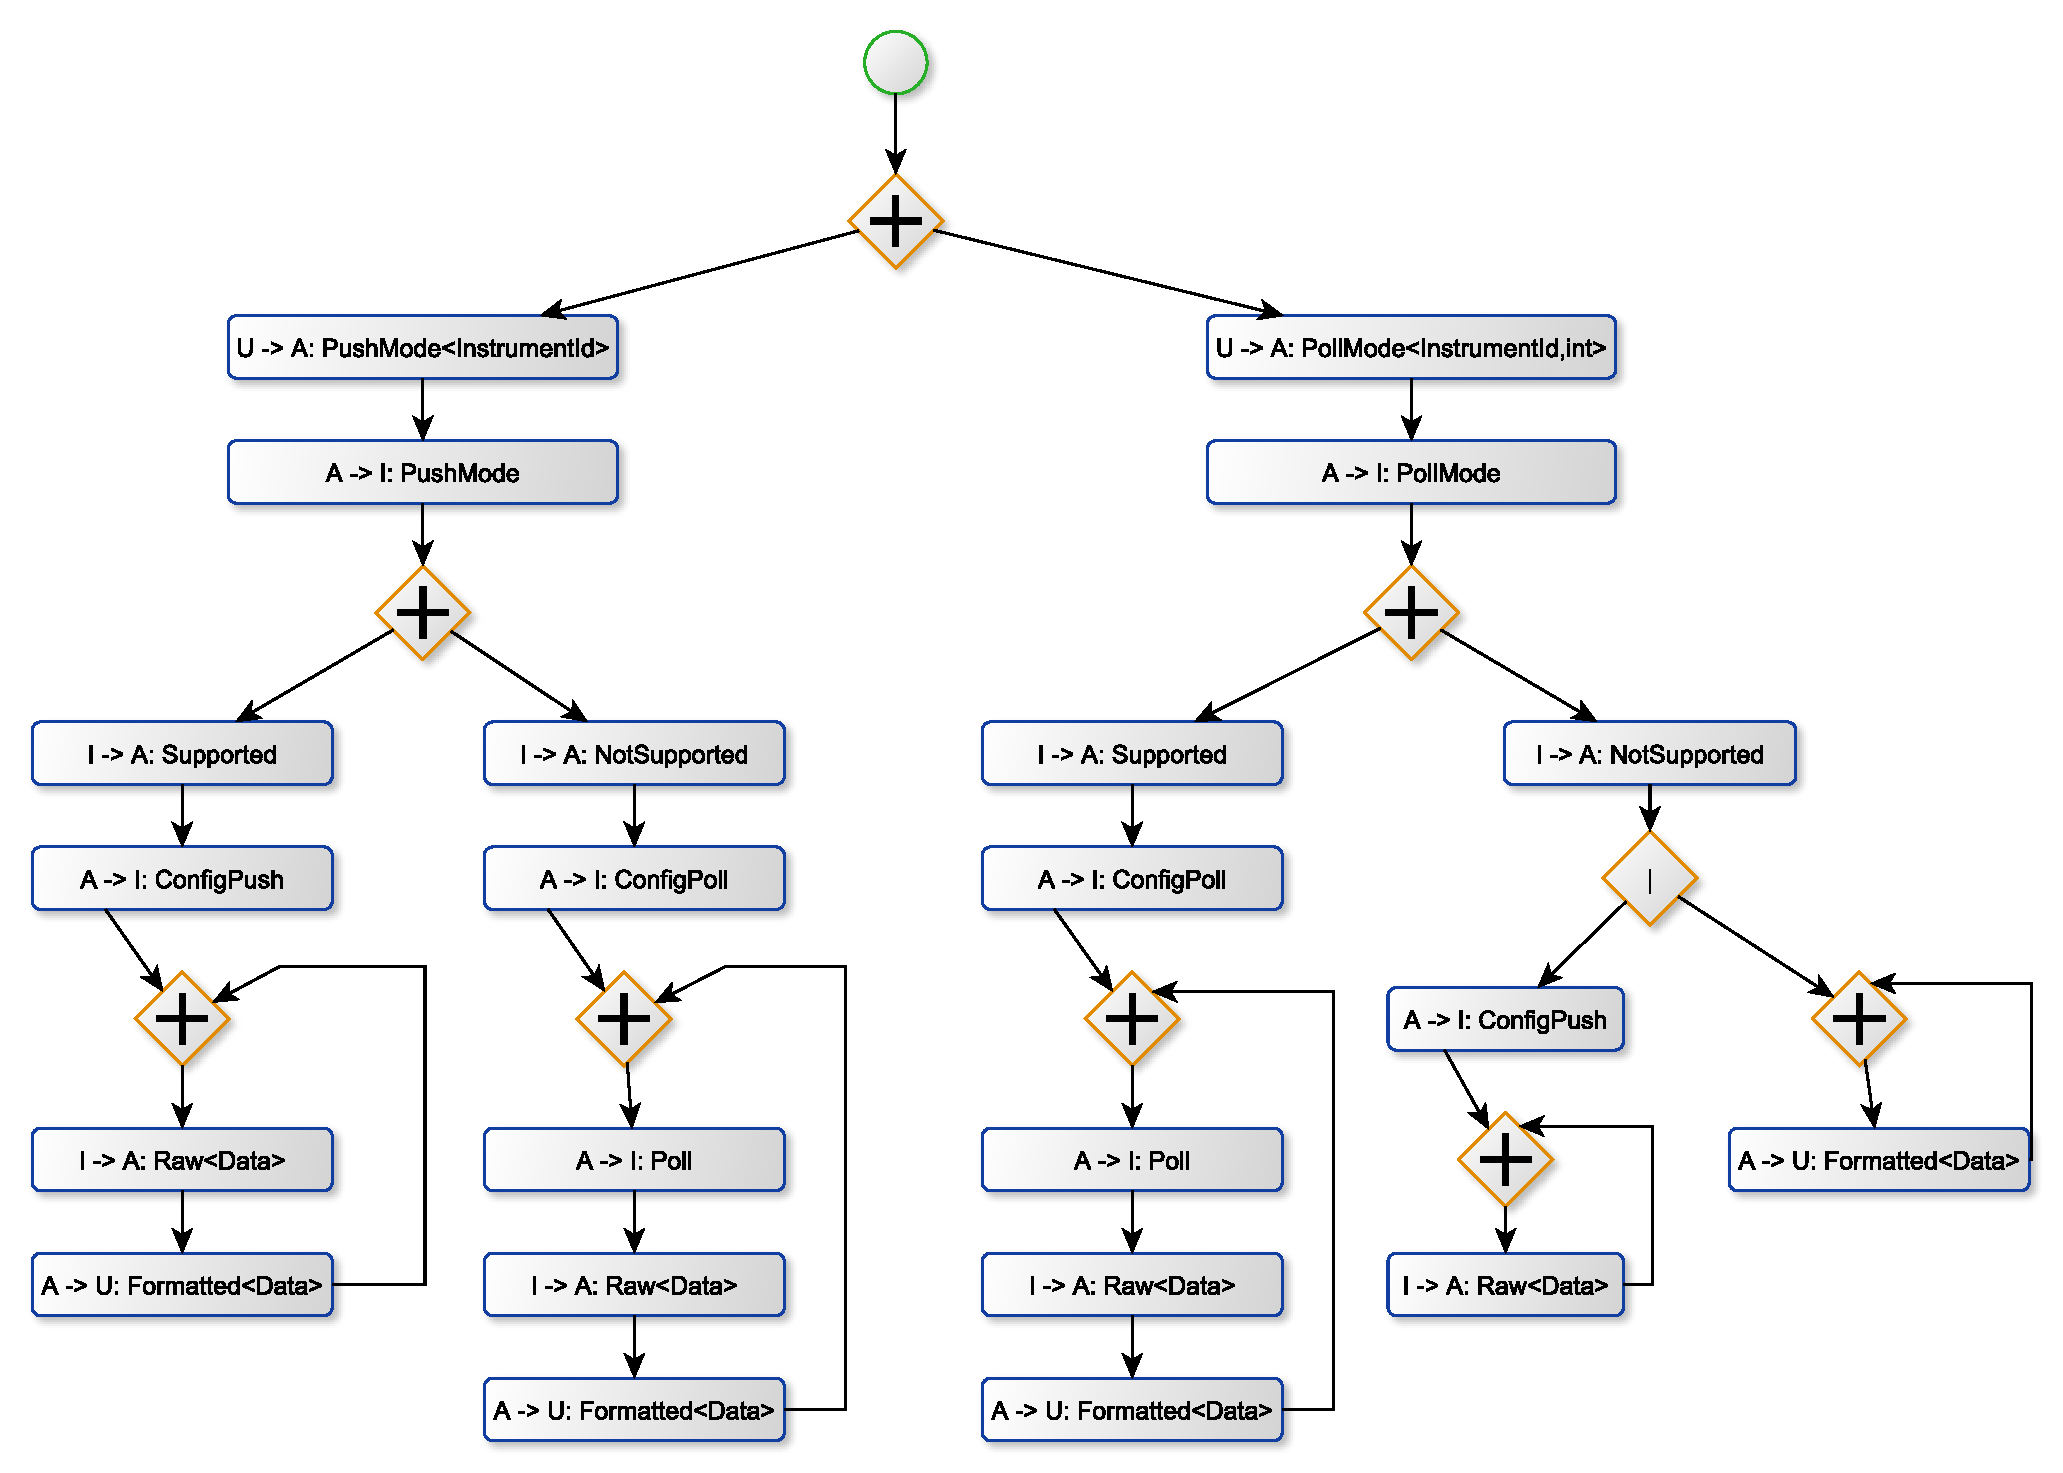
\includegraphics[scale=0.45]{ooi_graph}
\end{center}
\caption{The choreography for the OOI ``Acquire Data from Instrument'' use case}\label{fig:ooi_graph}
\end{figure}

As we are interested in global protocol, we present in Figure \ref{fig:ooi_example1} the translation of this use case into global types as defined in generalised mutliparty session types. We can easily see the exact match between the graph representation and the global protocol: indeed, edges are variables and nodes are transitions.\\
\begin{figure}[h]
\begin{tabular}{rcrcl}
G =& def & $x_{0}$ &=& $x_{push} + x_{poll}$\\
&& $x_{push}$ &=& U $\rightarrow$ A: PushMode$\langle$ InstrumentId $\rangle ; x_{push1}$\\
&& $x_{push1}$ &=& A $\rightarrow$ I: PushMode ;$ x_{push2}$\\
&& $x_{push2}$ &=& $ x_{pushsup} + x_{pushnsup}$\\
&& $x_{pushsup}$ &=& I $\rightarrow$ A: Supported$ ; x_{pushsup1}$\\
&& $x_{pushsup1}$ &=& A $\rightarrow$ I: ConfigPush$ ; x_{pushsup2}$\\
&& $x_{pushsup2} + x_{pushsup4}$ &=& I $\rightarrow$ A: Raw$\langle$ Data $\rangle ; x_{pushsup3}$\\
&& $x_{pushsup3}$ &=& A $\rightarrow$ U: Formatted$\langle$ Data $\rangle ; x_{pushsup4}$\\
&& $x_{pushnsup}$ &=& I $\rightarrow$ A: NotSupported$ ; x_{pushnsup1}$\\
&& $x_{pushnsup1}$ &=& A $\rightarrow$ I: ConfigPoll$ ; x_{pushnsup2}$\\
&& $x_{pushnsup2} + x_{pushnsup5}$ &=& A $\rightarrow$ I: Poll$ ; x_{pushnsup3}$\\
&& $x_{pushnsup3}$ &= & I$\rightarrow$ A: Raw$\langle$ Data $\rangle ; x_{pushnsup4}$\\
&& $x_{pushnsup4}$ &=& A $\rightarrow$ U: Formatted$\langle$ Data $\rangle ; x_{pushnsup5}$\\
&& $x_{poll}$ &=& U $\rightarrow$ A: PollMode$\langle$ InstrumentId, int $\rangle ; x_{poll1}$\\
&& $x_{poll1}$ &=& A $\rightarrow$ I: PollMode ;$ x_{poll2}$\\
&& $x_{poll2}$ &=& $ x_{pollsup} + x_{pollnsup}$\\
&& $x_{pollsup}$ &=& I $\rightarrow$ A: Supported$ ; x_{pollsup1}$\\
&& $x_{pollsup1}$ &=& A $\rightarrow$ I: ConfigPoll$ ; x_{pollsup2}$\\
&& $x_{pollsup2} + x_{pollsup5}$ &=& A $\rightarrow$ I: Poll$ ; x_{pollsup3}$\\
&& $x_{pollsup3}$ &=&  $\rightarrow$ A: Raw$\langle$ Data $\rangle ; x_{pollsup4}$\\
&& $x_{pollsup4}$ &=& A $\rightarrow$ U: Formatted$\langle$ Data $\rangle ; x_{pollsup5}$\\
&& $x_{pollnsup}$ &=& I $\rightarrow$ A: NotSupported$ ; x_{pollnsup1}$\\
&& $x_{pollnsup1}$& = &$ x_{pollnsup2}\ |\ x_{pollnsup3}$\\
&& $x_{pollnsup2}$ &=& A $\rightarrow$ I: ConfigPush$ ; x_{pollnsup4}$\\
&& $x_{pollnsup4} + x_{pollnsup5}$ &=& I $\rightarrow$ A: Raw$\langle$ Data $\rangle ; x_{pollnsup5}$\\
&& $x_{pollnsup3} + x_{pollnsup6}$ &=& A $\rightarrow$ U: Formatted$\langle$ Data $\rangle ; x_{pollnsup6}$\\
& in $x_{0}$&&&\\
\end{tabular}
\caption{The global protocol for the OOI ``Acquire Data from Instrument'' use case\label{fig:ooi_example1}}
\end{figure}
$x_0$ represents the initial state.\\
$ x_{0}$ = $x_{push} + x_{poll}$ is a choice, that is U will make the choice between continuing with $x_{push}$ or $x_{poll}$.\\
$ x_{pushsup2} + x_{pushsup4}$ = I $\rightarrow$ A: Raw$\langle$Data$\rangle ; x_{pushsup3}$ is a merge and in this case expresses recursion.\\
$x_{pollnsup1}$ = $ x_{pollnsup2}\ |\ x_{pollnsup3}$ is a fork to model interleaving of actions at $x_{pollnsup2}$ and $x_{pollnsup3}$.

Once global types have been established, we can write the corresponding safe program, using Scribble as language. The program for this example is given in Figure \ref{fig:ooi_example2}. Then there is a tool to deduce from the Scribble program the safe local programs.

Therefore the missing part of the tool chain is the graph representation of the globol protocol, the development of which will be our contribution. From now on, we will review the different calculus to explain the origin of generalised multiparty session types.

\newcommand{\MYPARAGRAPH}[1]{\paragraph{\textnormal{\textbf{#1}}}}

\definecolor{dkblue}{rgb}{0,0.1,0.5}
\definecolor{dkgreen}{rgb}{0,0.4,0}
\definecolor{dkred}{rgb}{0.4,0,0}


\newcommand{\CODESIZE}{\small}
%\newcommand{\CODESIZE}{\smaller}
\newcommand{\CODESTYLE}{\ttfamily}

\lstset%
{%
	%breakautoindent=true,
	%breaklines=true,
	captionpos=b,
	%columns=fixed,
	columns=flexible, % doesn't give proper space sizes, but fixed is much too fat
	%commentstyle=\itshape\CODESIZE\color{purple},
	commentstyle=\CODESTYLE\footnotesize\color{purple},
	escapeinside={*@}{@*},
	%extendedchars=true,
	float=hbp,
	frame=none,
	% identifierstyle=\color{black},
	language=Java,
	mathescape=true,
	numbers=none, % OLD: Numbers "on" by default: listings inside e.g. tabulars don't seem to work if we give parameters. % Maybe inline \lstset will help?
	numberstyle=\tiny,
	showspaces=false,
	showstringspaces=false,
	showtabs=false,
	stringstyle=\color{teal},
	tabsize=2%, % For some reason, has to be size 9 (equivalently 9 manual spaces) to match \noindent\CODE{12345678}. % maybe due to columns setting
	%xleftmargin=\DEFAULTXLEFTMARGIN % Roughly following the default tabsize.
}

\newcommand{\CODE}[1]{\texttt{\CODESIZE#1}} % Inline code listing (no additional formatting). convention: no colour formatting for inline code.
\newcommand{\GREYCODE}[1]{\CODE{
	%\color{gray}{#1}}} % Problem: braces aren't the same style
	\color{black}{#1}}} % Problem: braces aren't the same style
\newcommand{\SJCODE}[1]
{%
	\lstinline[style=SJ]+#1+%
}

\lstnewenvironment{CODELISTING}% % Listing without numbers or keywords; other parameters as above.
{%
	\onehalfspacing
	%\singlespacing
	\lstset%
	{%
		basicstyle=\CODESTYLE\footnotesize,
		keywordstyle=\CODESTYLE\footnotesize,
		%numbers=none,
		%tabsize=4 % Trying to keep tabsize a variable parameter isn't compatible with indentation conventions. The tabsize is now different to the SJBNF listing, but keep the default xleftmargin to align with BNF listings.
	}
}%
{%
	\doublespacing % Based on the settings of icthesis.sty
}

\lstdefinestyle{SJ}%
{%
	basicstyle   = \CODESTYLE\footnotesize,
	keywordstyle=[1]{
	%\bfseries
	\!\!\!\color{dkblue}
	\CODESTYLE\footnotesize},
	keywordstyle=[2]{
	%\bfseries
	\!\!\!\color{dkgreen}
	\CODESTYLE\footnotesize},
	%numbers     = none,
	%tabsize      = 4, % Same as the tabsize in the CODELISTING environment.
        moredelim=*[s][\footnotesize\color{dkgreen}]{<}{>},
        morekeywords =
	[1]{%
		%terminal, non, extend, RESULT
		protocol, role, choice, at, or, from, to, rec, parallel,
                and, interruptible, by, finish, continue, global, local, self, within
	},
	morekeywords =
	[2]{%
                int,Data,
	%	noalias,
	%	protocol,
	%	cbegin, sbegin, rec, end,
	%	using,
	%	accept, request,
	%	send, receive, receiveInt, receiveDouble, receiveFloat, receiveByte, receiveLong,
	%	outbranch, inbranch, outwhile, inwhile, recursion, recurse,
	%	spawn,
	%	typecase, when,
	%	register, select
	},
       literate={>=}{$\geq\ $}{2}{<=}{$\leq\ $}{2}
}

\lstnewenvironment{SJLISTING}%
{
	\lstset{style=SJ}
}
{
}


%%
% General latex stuff
%
\newcommand{\REF}[1]{\S\,\ref{#1}}

%%
% General code stuff
%
%\newcommand{\CODE}[1]{{\small \texttt{#1}}}
\newcommand{\OPASSIGN}{\, \CODE{:=} \,}
%\newcommand{\OPEQ}{\, \CODE{==} \,}
\newcommand{\OPEQ}{\ensuremath{=}}
\newcommand{\OPDEC}{\CODE{--}}
\newcommand{\OPINC}{\CODE{++}}
\newcommand{\OPSEQ}{\CODE{;}}
\newcommand{\OPNOT}{\ensuremath{\neg}}

%%
% General maths stuff
%\lstnewenvironment{SJLISTING}%
\newcommand{\OLINE}[1]{\ensuremath{\overline{#1}}}  % Overhead line
\newcommand{\SET}[1]{\ensuremath{\{ #1 \}}}         % Set braces
\newcommand{\FUN}[2]{\ensuremath{\mathsf{#1}(#2)}}  % Function call

%%
% General process stuff
%
\newcommand{\KWORD}[1]{\ensuremath{\mathsf{#1}}}
\newcommand{\DTYPE}[1]{\ensuremath{\mathtt{#1}}}  % Data type
\newcommand{\DVAL}[1]{\ensuremath{\mathtt{#1}}}   % Data value
\newcommand{\PPAR}{\ensuremath{\, | \,}}
\newcommand{\PPARGROUP}[1]{\ensuremath{(#1)}}
\newcommand{\PIF}{\ensuremath{\KWORD{if}}}
\newcommand{\PTHEN}{\ensuremath{\KWORD{then}}}
\newcommand{\PELSE}{\ensuremath{\KWORD{else}}}
\newcommand{\PNIL}{\ensuremath{\mathbf{0}}}
\newcommand{\EMPTY}{\ensuremath{\epsilon}}

%%
% General session types stuff
%
\newcommand{\LAB}[1]
	{\ensuremath{#1}}            % "Meta" label: "l"
\newcommand{\LABVAL}[1]
	{\ensuremath{\mathtt{#1}}}   % "Concrete" label: "quit"
\newcommand{\ROLE}[1]
	{\participant{#1}}           % Role/participant
\newcommand{\PARTY}[1]
	{\ensuremath{\mathsf{#1}}}   % Principal
\newcommand{\MSGlxS}[3]
	{\ensuremath{\MSGlx{#1}{#2\!:\!#3}}}  % lab(x:S)
\newcommand{\MSGlx}[2]
	{\ensuremath{#1 (#2)}}              % lab(x)  (variant needed to avoid ":")
\newcommand{\MSGlS}[2]
	{\MSGlx{#1}{#2}}                    % lab(S)
\newcommand{\BRANCH}[1]
	{\ensuremath{\SET{#1}}}         % Branch braces: {...}
\newcommand{\MUREC}[1]
	{\ensuremath{\mu \RECVAR{#1}}}  % Recursion prefix
\newcommand{\RECVAR}[1]
	{\ensuremath{\keyword{#1}}}     % Recursion var.

%%
% General session types stuff
%
\newcommand{\STATEVAR}[1]
	{\ensuremath{\mathtt{#1}}}                % State var.
\newcommand{\ROLEVAR}[2]
	{\ensuremath{\ROLE{#1} . \STATEVAR{#2}}}  % p.x
%\newcommand{\STATEDECL}[2]
	%{\ensuremath{#1 : \DTYPE{#2}}}
\newcommand{\STATEVARDECL}[2]
	%{\ensuremath{\STATEDECL{\STATEVAR{#1}}{#2}}}  % x : Nat
	{\ensuremath{\STATEVAR{#1} : \DTYPE{#2}}}      % x : Nat
\newcommand{\PARTYSTATEDECL}[2]
	{\ensuremath{\ROLE{#1}} : [#2]}                % p[x : Nat, ...]

%%
% Global types
%
\newcommand{\GSEP}{\ensuremath{.}}  % Global type separator
\newcommand{\GLOBAL}[1]
	{\ensuremath{\mathcal{#1}}}       % Global type name: G
\newcommand{\GLOBALi}[2]
	{\ensuremath{\GLOBAL{#1}_{#2}}}   % G_auction
\newcommand{\GSEND}[2]
	{\ensuremath{\ROLE{#1} \rightarrow \ROLE{#2} :}}  % p -> q:
%\newcommand{\GSEND}[5]
	%{\ensuremath{#1 \rightarrow #2 : \MSG{#3}{#4}{#5}}}

% Deprecated: use \BRANCH and \MUREC instead (same for both global and local)
\newcommand{\GBRA}[1]
	{\ensuremath{\SET{#1}}}         % Global branch braces: {...}
\newcommand{\GREC}[1]
	{\ensuremath{\mu \RECVAR{#1}}}  % Global recursion prefix

%%
% Global types for assertions/effects
%
\newcommand{\GLOBALDECL}[1]
	{\ensuremath{((#1))}}             % State var. decl. prefix
\newcommand{\LASS}[1]
	{\ensuremath{\langle #1 \rangle}}  % Left assertion: {...}
\newcommand{\LEFF}[1]
	{\LASS{#1}}                        % Left effect: {...}
\newcommand{\LASSEFF}[2]
	{\ensuremath{\LASS{#1,\, #2}}}     % Left assertion and effect: {..., ...}
\newcommand{\RASS}[1]
	{\ensuremath{\{ #1 \}}}            % Right assertion: <...>
\newcommand{\REFF}[1]
	{\RASS{#1}}                        % Right effect: <...>
\newcommand{\RASSEFF}[2]
	{\ensuremath{\RASS{#1,\, #2}}}     % Right assertion and effect: <..., ...>
\newcommand{\GRECtexA}[4]
	{\ensuremath{\MUREC{#1} \langle #2 \rangle (#3) \{ #4 \}}}
\newcommand{\GRECVARte}[2]
	{\ensuremath{\RECVAR{#1} \langle #2 \rangle}}

%%
% Local types
%
\newcommand{\LSEP}{\ensuremath{.}}  % Local type separator
\newcommand{\LOCAL}[1]
	{\ensuremath{\mathcal{#1}}}       % Local type name: L
\newcommand{\LOCALi}[2]
	{\ensuremath{\LOCAL{#1}_{#2}}}    % L_auction
\newcommand{\LSEND}[1]
	{\ensuremath{\ROLE{#1} \,!\,}}    % p!
\newcommand{\LRECV}[1]
	{\ensuremath{\ROLE{#1} \,?}}      % q!

%%
% Local types for assertions/effeacts
%
\newcommand{\LOCALDECL}[1]
	{\ensuremath{[#1]}}               % State var. decl. prefix
\newcommand{\LRECtexA}[4]
	{\GRECtexA{#1}{#2}{#3}{#4}}
\newcommand{\LRECVARte}[2]
	{\GRECVARte{#1}{#2}}

%%
% Session processes (1)
%
\newcommand{\POSEP}{\ensuremath{;}}  % After output prefixes
\newcommand{\PESEP}{\ensuremath{;}}  % Separator for effects
\newcommand{\PSEP}{\ensuremath{.}}   % Others: input prefixes, recursion, etc.
\newcommand{\PINIT}[1]
	{\ensuremath{\mathsf{#1}}}         % Initial process
\newcommand{\PINITi}[2]
	{\ensuremath{\mathsf{#1}_{#2}}}    % e.g. initial P_Server
%\newcommand{\PRUNT}
	%{\ensuremath{#1}}
\newcommand{\PREQ}[4]
	{\ensuremath{\OLINE{#1} \langle #2 [\ROLE{#3}] : \GLOBAL{#4} \rangle}}
                                                                % a~<x[p]:G>
\newcommand{\PACC}[4]
	{\ensuremath{#1 ( #2 [ \ROLE{#3} ] : \GLOBAL{#4} )}}          % a(x[p]:G)
\newcommand{\PSEND}[5]
	{\ensuremath{#1 [\ROLE{#2}, \ROLE{#3}] \,!\, \LAB{#4} \langle #5 \rangle}}
	                                                              % k[p,q]!l<e>
\newcommand{\PRECV}[3]
	{\ensuremath{#1 [\ROLE{#2}, \ROLE{#3}] \,?\,}}                % k[p,q]?
\newcommand{\PRECX}[1]
	{\ensuremath{\mu #1}}                            % mu X
\newcommand{\PRECXx}[2]
	{\ensuremath{\PRECX{#1} (#2)}}                   % mu X (x) ...
\newcommand{\PRECe}[1]
	{\ensuremath{\langle #1 \rangle}}                % ... <e>
\newcommand{\PRECVARX}[1]
	{\ensuremath{#1}}                                % X
\newcommand{\PRECVARXe}[2]
	{\ensuremath{\PRECVARX{#1} \langle #2 \rangle}}  % X<e>

% Deprecated: syntax change
\newcommand{\PRECx}[2]
	{\ensuremath{\MUREC{#1} (#2)}}
\newcommand{\PRECtx}[2]
	{\ensuremath{\MUREC{#1} (#2)}}      % mu t (x) ...
\newcommand{\PRECVARte}[2]
	{\GRECVARte{#1}{#2}}

%%
% Session processes (2)
%
\newcommand{\PNEWKW}{\KWORD{new}}
\newcommand{\PREGKW}{\KWORD{reg}}
\newcommand{\PINKW}{\KWORD{in}}
%\newcommand{\PWITHKW}{\KWORD{with}}
%\newcommand{\PINVITE}[2]
	%{\ensuremath{\mathtt{I}(\mathcal{#1}[\ROLE{#2}])}}          % I(G[p])
\newcommand{\PNEWs}[4]
	{\ensuremath{\PNEWKW\, (\AT{#1}{#2}, \ROLE{#3}) \,\PINKW\, #4}}  % new (s:G, p) in P
\newcommand{\PNEWa}[4]
	{\ensuremath{\PREGKW\, \AT{#1}{#2}[\ROLE{#3}] \,\PINKW\, #4}}
                                                        % new a:I(G[p]) in P
\newcommand{\PNEWp}[4]
	{\ensuremath{\PNEWKW\, \AT{#1}{#2} \,\KWORD{with}\, [#3] \,\PINKW\, #4}}
                                           % new \alpha:\Gamma with [P] in Q

% Deprecated: not needed
%\newcommand{\PJOINKW}{\KWORD{join}}
\newcommand{\PJOIN}[2]
	{\ensuremath{\KWORD{join}\, #1[#2]}}  % join s[p]

%%
% Session processes (3)
%
\newcommand{\PLOCK}
	{\ensuremath{\blacktriangledown \,}}
\newcommand{\PUNLOCK}
	{\ensuremath{\blacktriangle}}
\newcommand{\PGET}[2]
	{\ensuremath{#1 \OPASSIGN get(\STATEVAR{#2})}}  % x := get(f)
\newcommand{\PPUT}[2]
	{\ensuremath{put(#1, \STATEVAR{#2})}}           % put(f, e)
\newcommand{\PLRECV}[3]
	{#1 [\ROLE{#2}, \ROLE{#3}] \, ? \blacktriangledown}

%%
% Session processes (4)
%
\newcommand{\PSNET}[1]
	{\ensuremath{#1}}     % Static network: N
\newcommand{\PSNETi}[2]
	{\ensuremath{#1_{#2}}}
%\newcommand{\PDNET}[1]
	%{\ensuremath{\mathcal{#1}}}
\newcommand{\PICHAN}[2]
	{\ensuremath{\mathtt{I}(#1 [\ROLE{#2}])}}
\newcommand{\POCHAN}[2]
	{\ensuremath{\mathtt{O}(#1 [\ROLE{#2}])}}
\newcommand{\PNETQUEUE}[2]
	{\ensuremath{\langle #1 ; #2 \rangle}}

\newcommand{\RAYCOMMENT}[1]{~\\ \textbf{RAY:} #1}


\begin{figure}[p]
\centering
%-- message label uniqueness: only needed to make automata deterministic
%-- may also have enough width to use full role names

%import PushDataRequest, PollDataRequest, NoSampleAcquisition, OkSampleAcquisition, ConfiguringInstrument, InstrumentNotAvailable
%import InstrumentAvailable, ExpiredConfiguration, Data, ParsedData, StreamAddress, ParsedStreamAddress
\begin{tabular}{ll}
\begin{minipage}{9cm}
{\lstset{numbers=left}
\begin{SJLISTING}
// U is User, A is ION Agent, I is Instrument
global protocol DataAcquisition(role U, role A, role I) {
	try {		choice at U { *@\label{line:userchoiceopen}@*
						PushMode(InstrumentId) from U to A;
						PushMode from A to I;
						choice at I {
							Supported from I to A;
							ConfigPush from A to I;
							rec PUSH { *@\label{line:firstrecursion}@*
								Raw(Data) from I to A;
								Formatted(Data) from A to U;
								PUSH;
							}
						} or {
							NotSupported from I to A;
							ConfigPoll from A to I;
							rec POLL {
								Poll from A to I;
								Raw(Data) from I to A;
								Formatted(Data) from A to U;
								POLL;
						}	}
					} or { *@\label{line:userchoiceor}@*
						PollMode(InstrumentId, int) from U to A;
						PollMode from A to I;
						choice at I {
							Supported from I to A;
							ConfigPoll from A to I;
							rec POLL {
								Poll from A to I;
								Raw(Data) from I to A;
								Formatted(Data) from A to U;
								continue POLL;
							}
						} or { *@\label{line:pollnotsupportedopen}@*
							NotSupported from I to A;
							parallel {
								ConfigPush from A to I;
								rec PUSH {
									Raw(Data) from I to A;
									continue PUSH;
								}
							} and {
								rec POLL {
									Formatted(Data) from A to U;
									continue POLL;	}
						}	} *@\label{line:pollnotsupportedclose}@*
					} *@\label{line:userchoiceclose}@*
	} interrupt {
		Stop by U
}	}
\end{SJLISTING}}
\end{minipage}
%\caption{A Scribble protocol for the OOI Acquire Data from I Use Case service (part 1).\label{fig:ooi_example1}}
%\end{figure}
&
%\begin{figure}[t]
%\hspace{-15mm}
\end{tabular}
\caption{The Scribble global protocol for the OOI ``Acquire Data from Instrument'' use case\label{fig:ooi_example2}}
\end{figure}


\section{Session Types}

As we have seen in the introduction there is a need in distributed programming for a clear structure to express conversation.\\
A session is a structure to encapsulate a safe communication scheme between two or more peers in a context of distributed processes. A type system is associated to this structure in order to statically check the programs from the processes.
A session is introduced to describe a sequence of interactions between the processes.

As the case of two processes was first studied, we begin with exposing the binary session types to get the idea of session types. Then it has been extended to more than two processes with multiparty session types in order to express more complex interactions. Therefore we will continue with a detailed presentation of multiparty session.

\subsection{Binary Session Types}

\begin{table}[tb]
\centering
\begin{tabular}{rclr}
 \PP & ::=  &  request a(k) in \PP   &   {Session Request}\\
     & \sep & accept a(k) in \PP   &   {Session Acceptance}\\
     & \sep & \outS{\Ik}\e\PP &    {Data sending}\\
     & \sep & \inpS{\Ik}\x\PP &    {Data reception}\\
     & \sep & throw \Ik[\Ik']; \PP & {Channel Sending}\\
     & \sep & catch \Ik(\Ik') in \PP &  {Channel Reception}\\
     & \sep & \Ik $\vartriangleleft$ ;{\PP} & {Label Selection}\\
     & \sep & \Ik $\vartriangleright \{  l_{1}:{\PP}_{1} \| ... \|  l_{n}:{\PP}_{n} \} $ & {Label Branching}\\[1mm]
     & \sep & \ifthenelse{\e}{\PP}{\Q} & {Conditional Branch}\\
      & \sep & \PP \pc \Q  & {Parallel}\\
      & \sep & inact & {Inaction}\\
      & \sep & \nuc{\Iu}{\PP} & {Name/Channel Hiding}\\
      & \sep & \defD \PP & {Recursion}\\
      & \sep & \X[\e\Ik] & {Process Variables}
\\
\\[2mm]
\e   & ::= & \Ic & {Constant}  \\
&  \sep & \e+\e' \sep  \e-\e' \sep \e+\e' \sep\NOT{\e} $\ldots$x
&{Expression}\\
\DD   & ::= & \Ddef &{Declaration}\\
\end{tabular}
\ \vspace{1mm}
\caption{Syntax for user-defined processes}\label{tab:syntaxB}
\end{table}

The binary session types contains the expected communication features, as studied in the Models of Concurrent Computation course: value sending and receiving, recursion, choice of interactions. What is new is the session inititation and session delegation.

We take an example to explain in more details the syntax (Table \ref{tab:syntaxB}), operational semantics and typing system.
We consider the case of a client using the National Rail website to book a train ticket. The scenario is as follow:
\begin{itemize}
\item The client first choose the destination.
\item Then the service contact the right company to delegate the deal. The client will continue the transaction, unaware that he now communicates directly with the company.
\item The client and the company exchange date, price and money.
\end{itemize}

Here is the syntax for the system made up of one client, {\em Client}, the National Rail Services, {\em NRS}, and one of the companies, {\em Company}.\\
~~\\
def Client = request a(k) in  k $\vartriangleleft$ bristol;k!(date);k?(price);k!(money);inact\\
and NRS(u,v) = accept u(v) in k $\vartriangleright$ \{bristol:request c(k') in throw k'[v];NRS(u',v') $\| ...\|$ newcastle: ... \} \\
and Company = accept c(k') in catch k'[k] in k?(date);k!(price);k?(money);Company\\
in Client | NRS(a,k) | Company

The first line specifies that a client first requests a session withe the national rail services, then chooses a destination, here labelled Bristol, and finally sends the date, receives the corresponding price and sends the money before halting. The second line describes  the interactions from the national rail side: it accepts the request of session and then have a branching choice. We only specify the case for the label called Bristol: NRS requests a new session with the corresponding company and delegates the deal, before being available again for other interactions. The third line specifies that a company first accepts the request for a new session, then receives the delegation of the deal and finally operates the receiveing of the date, the sending of the price and the receiving of the money, before being available again.

Rather than exposing all the tables for operational semantics and typing system, that can be found in \cite{honda1998language,yoshida2007language}, we apply the rules to reduct our example.\\
Let call \PP ~the system above defined and D the declaration for recursion inside \PP, and apply to it the reduction rules.

\begin{tabular}{lclr}
\PP& $\rightarrow$ &def D in ($\nu$ k) ( k $\vartriangleleft$ bristol;k!(date);k?(price);k!(money);inact | & [Link]\\
&& k $\vartriangleright$ \{bristol:request c(k') in throw k'[k];NRS(u',v') $\| ...\|$ newcastle: ... \}) |&  \\
&&accept c(k') in catch k'[k] in k?(date);k!(price);k?(money);Company&  \\
& $\rightarrow$  & def D in ($\nu$ k) (k!(date);k?(price);k!(money);inact | &[Label]\\
&& request c(k') in throw k'[k];NRS(u',v')  )|&\\
&&accept c(k') in catch k'[k] in k?(date);k!(price);k?(money);Company&\\
& $\rightarrow$  & def D in ($\nu$ k) (k!(date);k?(price);k!(money);inact | & [Link]\\
&& ($\nu$ k')(throw k'[k];NRS(u',v') | &\\
&&catch k'[k] in k?(date);k!(price);k?(money);Company))&\\
& $\rightarrow$  & def D in ($\nu$ k) (k!(date);k?(price);k!(money);inact | & [Pass]\\
&& ($\nu$ k')(NRS(u',v') |  k?(date);k!(price);k?(money);Company))&\\
& $\rightarrow$  & def D in ($\nu$ k) (k?(price);k!(money);inact |  ($\nu$ k')(NRS(u',v') |  &\\
&&k!(price);k?(money);Company))& [Com]\\
& $\rightarrow$  & def D in ($\nu$ k)( k!(money);inact | ($\nu$ k')(NRS(u',v') |  k?(money);Company))&[Com]\\
& $\rightarrow$  & def D in ($\nu$ k) (inact |  ($\nu$ k')(NRS(u',v') | Company))& [Com]\\
& $\equiv$  & def D in (NRS(u',v') | Company) & \\
\end{tabular}
\\

Besides the specified reduction rules we used [Def] at each step and [Str] at the second [Link] step in order to put the third part inside ($\nu$ k).

The process \PP~is also typable with respect to the typing system. We give here two steps of this typing:
\[ \der \Ga { k \vartriangleleft bristol;k!(date);k?(price);k!(money);inact}\D,k:\oplus \{ bristol:![nat];?[nat];![nat];end\}\]
\[ \der \Ga {catch~ k'[k] in~ k?(date);k!(price);k?(money);inact}\D,k':?[~ ![nat];?[nat];![nat];end~ ];end\]

Therefore binary session types allows to express complex communication structure between two peers and to ensure its safety. Nevertheless, in a real world context, communication usually involves more than two entities. To solve this issue, one can first think of modelling interactions between more than two processes using binary session types for each pair of them. However it appears to remove the desired clarity of the structure. Furthermore it can not express the situation as a whole but only separate interactions. That is why researchers introduce multiparty session types.

\subsection{Multiparty Session Types}

\subsubsection{Overview}

A multiparty session describe the interactions between several processes. Besides specifying the user-defined processes involved in a session, we have to define, at a higher level, a global protocol that ensures the coherence of the session. The type system allows specifying these two levels: first there is a global type and then projections of this global type to each endpoint processes. \\
In multiparty session programming, a developer will have to define the global type and the user-defined processes. The key step in the methodology consists then of checking the correspondence between the projections from the global type and the type of the endpoint programs.

With respect to the procedure, we get several properties: type safety, session fidelity, progress, linearity. Also the structure of sessions makes it possible to deal with interferences and interleaving of interactions among participants.

To describe with more details and more formally what is explained above, we look at the example of the three buyers protocol and then introduce syntax, operational semantics and a type system, as defined in \cite{coppoglobal}.

\subsubsection{The three buyers protocol example}

We first introduce the calculus through the example of the three-buyer protocol,
%in order to demonstrate the new features
which includes the expected communiaction features, as well as session-multicasting and
dynamically merging two conversations.
% The following figure depicts the interaction between the four
% parties involved: three buyers (Buyer1, 2 and 3) and
% the book seller (Seller). Buyer1, Seller and Carol are initially unknown
% to each other but later communicate directly (transparently to
% Buyer1 and Seller) through the use of delegation, to enable dynamic
% merging of two conversations.
The overall scenario  proceeds as follows.
\begin{enumerate}
\item
Alice sends a book title to Seller, then Seller sends back a quote
to Alice and Bob. Then Alice tells Bob how much she can contribute.

\item
If the price is within Bob's budget, Bob notifies both Seller and
Alice he accepts, then sends his address, and Seller sends back the
delivery date.

\item
If the price exceeds the budget, Bob asks Carol to collaborate
together by establishing a new session. Then Bob sends how much
Carol must pay, then {\em delegates} the remaining interactions with
Alice and Seller to Carol.

\item
If the rest of the price is within Carol's budget, Carol accepts the
quote and notifies Alice, Bob and Seller, and continues the rest of
the protocol with Seller and Alice transparently, {\em as if she were
Bob}. Otherwise she notifies Alice, Bob and Seller to quit the
protocol.\vspace{-2mm}
\end{enumerate}

Figure~\ref{fig:threebuyers} depicts an execution of the above
protocol where Bob asks Carol to collaborate (by delegating the
remaining interactions with Alice and Seller) and the transaction
terminates successfully.

\begin{figure}[tb]
\begin{center}
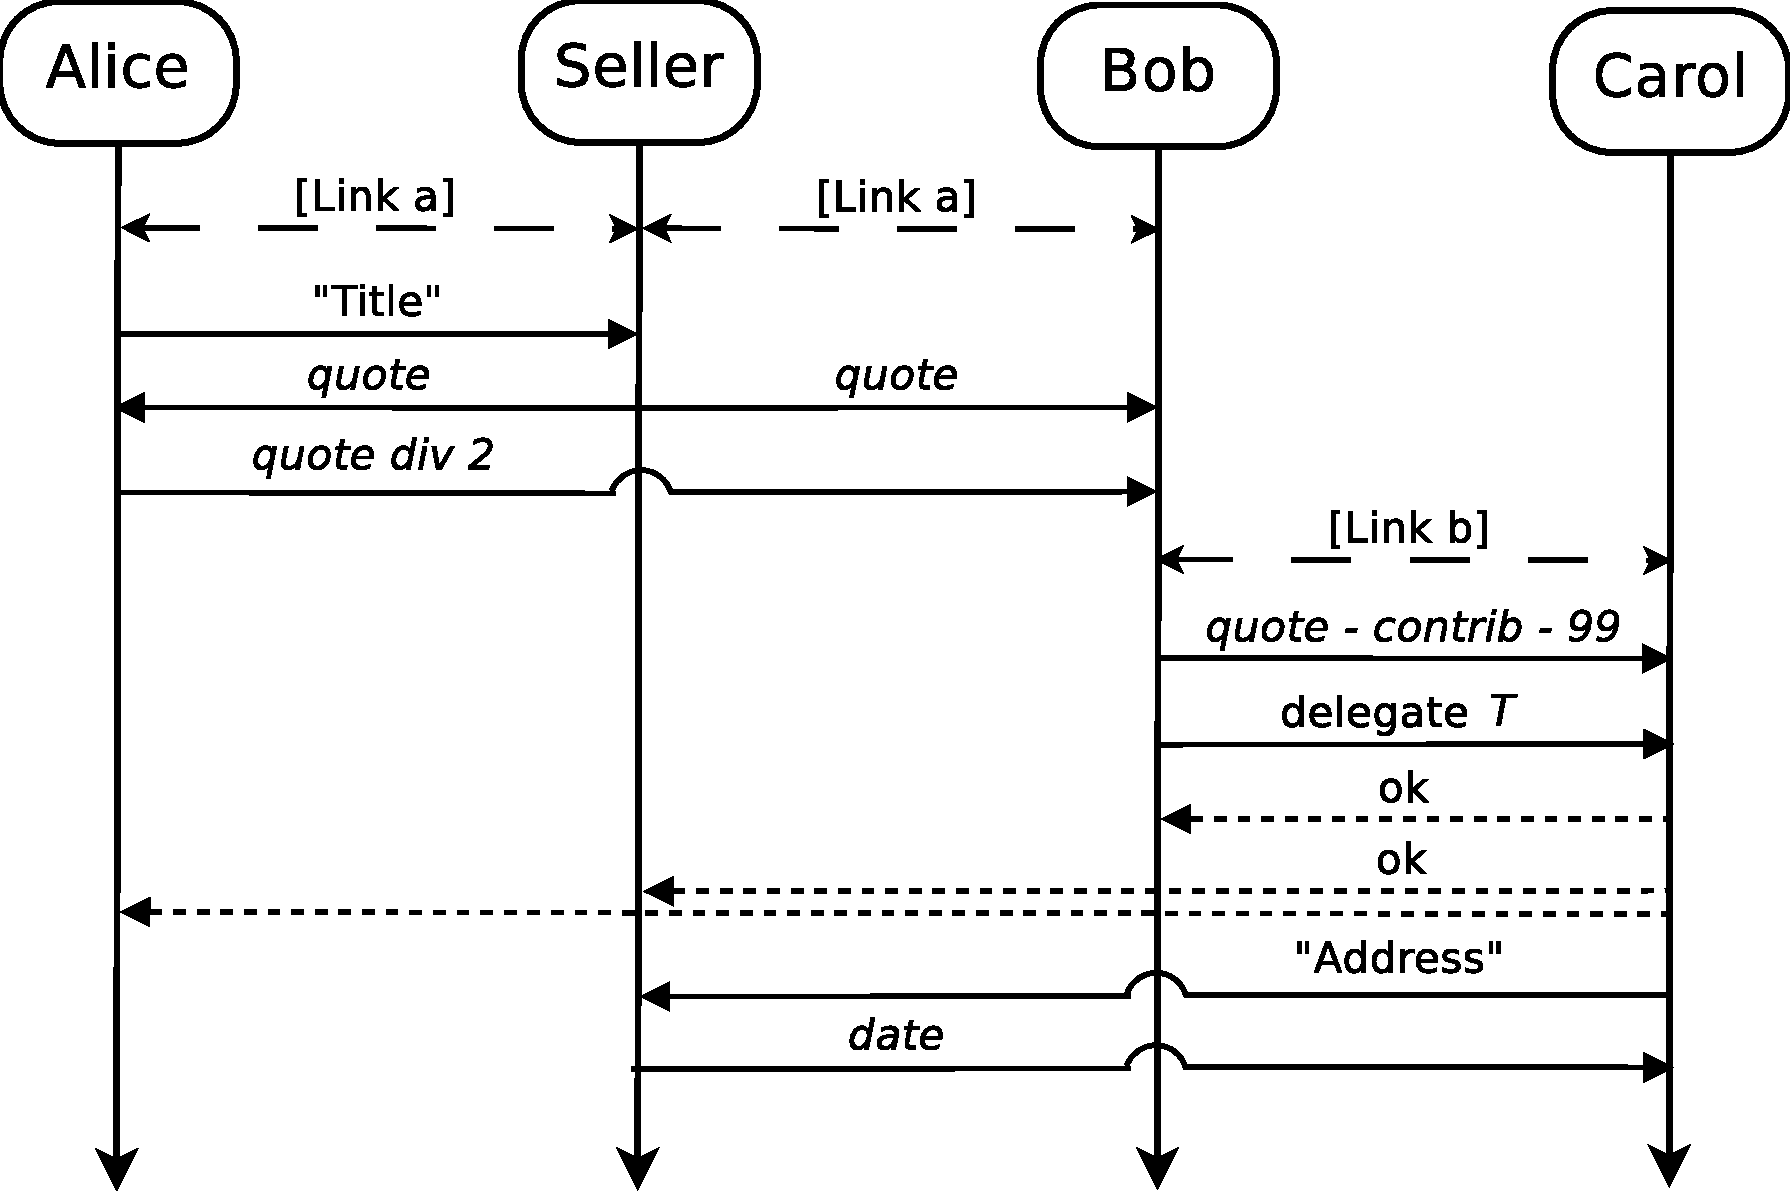
\includegraphics[scale=0.25]{three_buyer_protocol}
\end{center}
\caption{The three buyer protocol interactions}\label{fig:threebuyers}
\end{figure}

Then multiparty session programming consists of two steps:
specifying the intended communication protocols using global types,
and implementing these protocols using processes. The specifications
of the three-buyer protocol are given as two separated global types:
one is $G_a$  among Alice, Bob and Seller and the other is $G_b$
between Bob and Carol. We write principals with legible symbols
though they will actually be coded by numbers: in $G_a$
we have  $\participant{A}=1$,
$\participant{B}=2$, and $\participant{S}=3$,
while in $G_b$ we have $\participant{B}=2$, $\participant{C}=1$.\\[0.5mm]
\newcommand{\nm}[1]{{\texttt{\scriptsize #1.}}}

{\small
$
\begin{array}{ll}
G_a =&  G_b =\\
\begin{array}{llllll}
 \nm{1}& \participant{A} & \redsym & \participant{S}: & \langle \kf{string}\rangle.\\
  \nm{2}&\participant{S}  & \redsym & \{\participant{A},\participant{B}\}: & \langle \mathsf{int}\rangle .\\
  \nm{3}&\participant{A} & \redsym & \participant{B}:& \langle \mathsf{int}\rangle .\\
  \nm{4}&\participant{B} & \redsym & \{\participant{S},\participant{A}\}: & \{\mathsf{ok:}
 \participant{B} \redsym \participant{S}:\langle \kf{string}\rangle.\\
 \nm{5}& & & & \quad\quad \ \participant{S} \redsym
\participant{B}:
\langle \kf{date}\rangle ;\End\\
\nm{6} & & & & \ \mathsf{quit}: \End\}\\
\\
\end{array}
&
\begin{array}{llllll}
 \nm{1} & \participant{B}& \redsym & \participant{C}:&\langle \kf{int}\rangle .\\
 \nm{2}      &\participant{B}& \redsym & \participant{C}:&\langle T \rangle .\\
 \nm{3}     &\participant{C}& \redsym & \participant{B}: &
\{\mathsf{ok}:
\End, \quad \mathsf{quit}: \End\}.\\[1mm]
 & & & & \hspace{-1.8cm}
T=\\
 & & & & \hspace{-1.8cm}\
\oplus \langle\{\participant{S},\participant{A}\},\\
 & & & & \hspace{-1.8cm} \  \ \ \ \ \{\mathsf{ok}:!\langle
\participant{S},\kf{string}\rangle; ?\langle
\participant{S},
\kf{date}\rangle;
\End,\\
 & & & & \hspace{-1.8cm} \ \ \ \ \ \ \mathsf{quit}: \End\}\rangle\\[0.5mm]
\end{array}
\end{array}
$\\[0.5mm]
}

The types give a global view of the two
conversations, directly abstracting the scenario given by the
diagram. In $G_a$, line 1 denotes $\participant{A}$ sends a
string value to $\participant{S}$. Line 2 says $\participant{S}$
multicasts the same integer value to $\participant{A}$ and
$\participant{B}$ and line 3 says that $\participant{A}$ sends an integer to
$\participant{B}$. In lines 4-6 $\participant{B}$ sends either
$\mathsf{ok}$ or $\mathsf{quit}$ to $\participant{S}$ and
$\participant{A}$. In the first case $\participant{B}$ sends a
string to $\participant{S}$ and receives a date from
$\participant{S}$, in the second case there are no further
communications.

Line 2 in $G_b$ represents the delegation of the capability
specified by the session type $T$ of channels (formally defined
later) from $\participant{B}$ to
$\participant{C}$ (note that \participant{S} and
\participant{A} in $\T$ concern the session on \Ia).

Figure~\ref{tbe} gives the code, associated to $G_a$ and $G_b$, for
\participant{S,\,A,\,B} and \participant{C} in a ``user'' syntax
formally defined later\footnote{In the examples we will use
the following font conventions: variables (bound by an input action) are in
\textit{italics} and constants are in
\constf{sans serif}; string literals are in \texttt{monospace} font and double
quoted. }:
\begin{figure}
\begin{tabular}{rcl}
\participant{S} & $=$ & $\bar{a}[3](y_3).y_3?(\textit{title});
y_3!\langle \constf{quote} \rangle; y_3\&
\{\mathsf{ok}:y_3?(\textit{address}); y_3!\langle \constf{date}
\rangle; \inact, \ \mathsf{quit}: \inact\}$
\\[2mm]
\participant{A} & $=$ & $a[1](y_1).y_1!\langle \texttt{"Title"} \rangle;
y_1?(\textit{quote});y_1!\langle \textit{quote} \ \mathsf{div} \
2\rangle; y_1\& \{\mathsf{ok}:\inact, \ \mathsf{quit}: \inact\}$
\\[2mm]
\participant{B} &  $=$ & $a[2](y_2).y_2?(\textit{quote}); y_2?(\textit{contrib});$\\
   &     & \indent $\mathsf{if}~(\textit{quote - contrib} < 100)
 ~\mathsf{then}~\ y_2 \oplus \mathsf{ok}; y_2!\langle
 \texttt{"Address"}\rangle;y_2?(\textit{date});  \inact$\\
& &  \indent $\mathsf{else}~\sr\Ib 2{\z_2
}{\z_2
!\langle
\textit{quote - contrib - }99\rangle; \z_2
!\langle\! \langle y_2
\rangle\!\rangle ; z_2
\& \{\mathsf{ok}: \inact, \ \mathsf{quit}: \inact\}}$\\[2mm]
\participant{C} &  $=$ &  $\sa \Ib 1 {z_1 }{\z_1 ?(x); \z_1
?(\! (t)\!)};$\\
   &      & $%\nind
 \mathsf{if}~(x < 100)~\mathsf{then}~z_1
\oplus \mathsf{ok};
t \oplus \mathsf{ok}; t!\langle
\texttt{"Address"}\rangle;t?(\textit{date}); \inact$\\ & & % \nind
$\mathsf{else}~z_1
\oplus \mathsf{quit};t \oplus \mathsf{quit}; \inact$
\end{tabular}\\[0.5mm]
\caption{The three buyer example}\label{tbe}
\end{figure}

Session name $\Ia$ establishes the session corresponding to
$\G_\Ia$.
\participant{S} initiates a session involving three bodies as third participant by
$\bar{a}[3](y_3)$: \participant{A} and \participant{B} participate
as first and second participants by $a[1](y_1)$ and
$a[2](y_2)$, respectively. Then \participant{S}, \participant{A} and
\participant{B} communicate using the channels $y_3$, $y_1$ and
$y_2$, respectively. Each channel $\y_\p$ can be seen as a
port connecting participant $\p$ with all other ones; the
receivers of the data sent on $\y_\p$ are specified by the global
type (this information will be included in the runtime code). The
first line of $\G_\Ia$ is implemented by the input and output
actions $y_3?(\textit{title})$ and $y_1!\langle \texttt{"Title"}
\rangle$. The last line of $\G_\Ib$ is implemented by the branching
and selection actions $z_2\& \{\mathsf{ok}: \inact, \ \mathsf{quit}:
\inact\}$ and $z_1\oplus \mathsf{ok}$, $z_1\oplus \mathsf{quit}$.

In \participant{B}, if the quote minus \participant{A}'s
contribution exceeds 100\euro\ (i.e., $\textit{quote - contrib} \geq
100$), another session  between \participant{B} and
\participant{C} is established dynamically through shared name
$\Ib$. The delegation is performed by passing the channel $y_2$ from
\participant{B} to \participant{C} (actions $\z_2!\langle\!
\langle y_2 \rangle\!\rangle$ and $\z_1?(\! (t)\!)$), and so the
rest of the session is carried out by \participant{C} with
\participant{S} and \participant{A}. 

This example illustrates how multiparty session types is used for such a protocol and garantees safe communication.\\

\subsubsection{Syntax and Operational semantics}

The real improvement in multiparty session types, compared to binary session types, is the notion of global protocol, which will be used as a choreography for the whole system. Ths syntax for global protocols can be found in \cite{coppoglobal}.
The grammar for processes, ranged over by $\PP,\Q\dots$, and for expressions, ranged over by $\e,\e',\dots$, similar to the binary session case, is given by the Table~\ref{tab:syntaxM}.\\
The rules for operational semantics are also from \cite{coppoglobal} and given in Tables~\ref{tab:strucCong}~\ref{tab:reduction}.

\begin{table}[tb]
\centering
\begin{tabular}{lll}
\begin{tabular}{rclr}
 \PP & ::=  & \sr\uu \pn\y\PP   &   {Multicast Request}\\
     & \sep & \sa\uu\p\y\PP   &   {Accept}\\
     & \sep & \outS{\y}\e\PP &    {Value sending}\\
     & \sep & \inpS{\y}\x\PP &    {Value reception}\\
     & \sep & \sdS{\y}{\z} \PP & {Session delegation}\\
     & \sep & \rdS{\y}{\z}\PP &  {Session reception}\\
     & \sep & \lselS{\y}{l}{\PP} & {Selection}\\
     & \sep & \lbranchS{\y} & {Branching}\\[1mm]
\uu & ::= & $\x$ \ \sep \Ia & {Identifier}\\
\va & ::= & \Ia \ \sep \true  \ \sep \false & {Value}\\
\end{tabular}
&
&
\begin{tabular}{rclr}
      & \sep & \ifthenelse{\e}{\PP}{\Q} & {Conditional}\\
      & \sep & \PP \pc \Q  & {Parallel}\\
      & \sep & \inact & {Inaction}\\
      & \sep & \nuc{\Ia}{\PP} & {Hiding}\\
      & \sep & \defD \PP & {Recursion}\\
      & \sep & \proccall{\X}{\e}{\y} & {Process call}
\\
\\[2mm]
\e   & ::= & \va \ \sep \x  \\
&  \sep & \AND{\e}{\e'} \sep \NOT{\e} $\ldots$
&{Expression}\\
\DD   & ::= & \Ddef &{Declaration}\\
\end{tabular}
\end{tabular}
\ \vspace{1mm}
\caption{Syntax for user-defined processes}\label{tab:syntaxM}
\end{table}

\begin{table}[tb]
\centering
\begin{tabular}{c}
  $P \Par \textbf{0}\equiv P\ \ \ \ \ P \Par Q\equiv Q \Par P\ \ \ \ \
  (P \Par Q) \Par R\equiv P \Par (Q \Par R)$\\
  \\
  $(\nu \cas)P \Par Q\equiv (\nu \cas)(P \Par Q)\ \ \ \ \ \ \text{if}\ \cas\notin
  \freen{\Q}$\\
  \\
  $(\nu \cas\cas')P\equiv (\nu \cas'\cas)P\ \ \ \ \ \ (\nu \cas)\textbf{0}\equiv \textbf{0}\ \
  \ \ \ \ \defD\textbf{0}\equiv \textbf{0}$\\
  \\
  $\defD(\nu \cas)P\equiv (\nu \cas)\defD\PP\ \ \ \ \ \ \text{if}\ \cas\notin
  \freen{D}$\\
  \\
  $(\defD\PP) \Par Q\equiv \defD{(P \Par Q)}\ \ \ \ \ \ \text{if}\ \dpv{D}\cap
  \fpv{Q}=\emptyset$\\
  \\
  $\defD(\defDp\PP)\equiv \defIn{\AND{D}{D'}}\PP\ \ \ \ \ \ \text{if}\
  \dpv{D}\cap \dpv{D'}=\emptyset$\\
  \\
   $\mqueue{\s}{
   \qhead
    {
        \qcomp
        {\trival{z}{\pset}{\q}}
        {\trival{z'}{\pset'}{\q'}}
    }
   } \equiv
   \mqueue{\s}{
   \qhead
    {
        \qcomp
        {\trival{z'}{\pset'}{\q'}}
        {\trival{z}{\pset}{\q}}
    }
   }$ 
   $\qquad \text{if $\pset \cap \pset'=\emptyset$ or $\q \ne \q'$}$\\
   \\
   $\mqueue{\s}{
   \qhead
    {
        {\trival{z}{ \pset}{\q}}
    }
   } \equiv
   \mqueue{\s}{
   \qhead
    {
        \qcomp
        {\trival{z}{\pset'}{\q}}
        {\trival{z}{\pset''}{\q}}
    }
   }$ 
   $\qquad \text{where $\pset = \pset' \cup \pset''$ and }\pset' \cap \pset''=\emptyset$
\end{tabular}
\caption{Structural equivalence (\cas\ ranges over \Ia, \s\ and $z$ ranges over
\at{\va}, \si\s\p\ and $l$.)}\label{tab:structcong}
\end{table}

\begin{table}[tb]
{\centering
\begin{tabular}{cr}
\\
         $\sa\Ia {1}{\y_1}{\PP_1}
        \pc...\pc\sr\Ia n{\y_n}{\PP_n}$
         $\redsym (\nu \s)(
        \PP_{1}\sub{\si\s {1}}{\y_{1}} \pc ...\pc
        \PP_n\sub{\si \s {n}}{\y_n}\pc s : \eq)$  & [Link]
\\[2mm]
    \red{\out{\si{\s}{\p}}{\e}{\p}{\PP} \pc \mqueue{\s}{\queue}}
    {\PP \pc\mqueue{\s}{\qtail{\valheap{\va}{\p}{\p}}}}
        \ \ (\at{\e}$\downarrow$\at{\va})
    & [Send]
\\[2mm]
    \red{\sd{\si{\s}{\p}}{\si{\s'}{\p'}}{\q}{\PP} \Par \mqueue{\s}{\queue}}
    {\PP \Par \mqueue{\s}{\qtail{\delheap{\si{\s'}{\p'}}{\q}{\p}}}}
    & [Deleg]
\\[2mm]
    \red{\lsel{\sii}{l}{\p}{\PP} \Par \stdqueue}
    {\PP \Par \qappend{\labheap{l}{\p}{\p}}}
    & [Label]
\\[2mm]
    $\inp{\sii}{\x}{\q}{\PP} \Par \qpop{\valheapp{\va}{\q}}$
    $\redsym \PP\subst{\ptilde{\va}}{\ptilde{\x}} \Par
    \mqueue{\s}{\queue}$ &
    [Recv]
\\[2mm]
    \red{\rd{\sii}{\y}{\q}{\PP} \Par \qpop{\delheap{\si{\s'}{\p'}}{\p}{\q}}}
    {\PP\subst{\si{\s'}{\p'}}{\y} \Par \stdqueue}
    & [Srec]
\\[2mm]
    \lbranch{\sii}{\q} \Par \qpop{\labheapp{l_{i_0
}}{\q}}
    $\redsym \PP_{i_0
} \Par \mqueue{\s}{\queue}$ \ \ $(i_0 \in I)$ & [Branch]
\\[2mm]
      \red{\ifthenelse{\e}{\PP}{\Q}}{\PP} \ \ \ $(\e \downarrow \true)$
    \quad
\red{\ifthenelse{\e}{\PP}{\Q}}{\Q} \ \ \ $(\e \downarrow \false)$
    &\hspace{-3mm}[If-T, If-F]
\\[2mm]
    $\DdefD (\proccallw{X}{\e}{\si\s\p} \Par \Q)$
    $\redsym \DdefD
    (\PP\subst{\at{\va}}{\at{\x}}\subst{\atw{\si\s\p}}{\at{\y}} \Par \Q)$\ \ \ \
    $(\ptilde{\e}\downarrow \at{\va})$ & \hspace{-3mm}[ProcCall]
\\[2mm]
  \red{\PP}{\PP'} \Implies \red{\nuc{\cas}{\PP}}{\nuc{\cas}{\PP'}}
\quad \quad \quad
  \red{\PP}{\PP'} \Implies \red{\PP \Par \Q}{\PP' \Par \Q}
  &\hspace{-3mm}[Scop,Par]
\\[2mm]
  \red{\PP}{\PP'} \Implies \red{\defD\PP}{\defD\PP'}
  & \hspace{-3mm}[Defin]
\\[2mm]
  $P\equiv P'\ \text{and}\ \red{P'}{Q'}\ \text{and}\ Q\equiv Q' \Implies
  \red{P}{Q}$ & \hspace{-3mm}[Str]
\\[2mm]
\end{tabular}}
\caption{Reduction rules}\label{tab:reduction}
\end{table}


\subsubsection{Typing System}

As we have introduced the notion of global protocol, we now define global types. As explained in the three buyers protocol, from the global type, one can deduce the local types thank to projections.

A \emph{global type}, ranged over by $G,G',..$
describes the whole conversation scenario of a
multiparty session as a type signature.
Its grammar is given below:

\begin{center}
\begin{tabular}{rclrrrclr}
Global \quad
 $\G$ & ::= & $\Gv\p\p\U{\G'}$  &\quad \quad \quad
& Exchange \quad & $\UT$   & ::= & $\ptilde{S}\ |\ \T$
\\
      & \sep & $\p\rightarrow\pset:\{l_i:\G_i\}_{i\in I}$ &
& Sorts \quad &

  $S$   & ::= & $\Bool\ |\ \ldots\ |\ G$ & \\
      & \sep & $\mu \ty.\G$  \sep $\ty$ \sep $\End$
\end{tabular}
\end{center}

We now define the local types of pure processes, called {\em session
types}.
While global types represent the whole protocol, session types
correspond to the communication actions, representing
sessions from the view-points of single participants.

\begin{center}
\small
\begin{tabular}{ll}
\begin{tabular}{lrclr}
  {Action} \quad \quad & $\T$ & ::= & \oT\UT{\pset};\T \
  & \emph{send}\\ &     & \sep & \iT \UT\p;\T &\emph{receive}\\
         &     & \sep & \seltype &\emph{selection}\\
         &     & \sep & \branchtype &\emph{branching}\\
\end{tabular}&
         \begin{tabular}{lrclr}
         &     & \sep & $\mu \ty.\T$ &\emph{recursive}\\
         &     & \sep & $\ty$  &\emph{variable}\\
         &     & \sep & $\End$ &\emph{end}\\
         &  $\;$   &  &\\
\end{tabular}
\\
\end{tabular}
\end{center}

The relation between session and global types is formalised by the
notion of projection. The {\em projection of \G\
onto \q} (\pro\G\q) is defined
by induction on \G:

\begin{quote}
{\small
$\pro{(\Gv\p\p\U{\G'})}\q=\begin{cases}
  \oT\UT{\pset};(\pro{\G'}\q)  & \text{if }\q=\p, \\
  \iT\UT{\p};(\pro{\G'}\q) & \text{if }\q\in\pset, \\
   \pro{\G'}\q & \text{otherwise}.
\end{cases}$\\
$\pro{(\p\rightarrow\pset:\{l_i:\G_i\}_{i\in I})}\q=$\\
\mbox{\qquad \qquad \qquad} $
 \begin{cases}
  \seltypeG & \text{if }\q=\p\\
  \branchtypeG& \text{if }\q\in\pset \\
   \pro{\G_1}\q  &\text{if }\q\not=\p,  \q\not\in\pset\text{ and }\\
     & \pro{\G_i}\q=\pro{\G_j}\q
   \text{ for all }i,j\in I.\end{cases}
$\\
$\pro{(\mu \ty.\G)}\q= \mu \ty.(\pro{\G}\q) \quad \pro\ty\q=\ty\quad\pro\End\q=
         \End$.\\[0.5mm]
}
\end{quote}

As an example, we list two of the projections of the global types $\G_\Ia$ and
$\G_\Ib$ of the first three-buyer protocol:
\[\begin{array}{lll}
 \pro{\G_\Ia}1&=& !\langle \{3\},\kf{string}\rangle;?( 3,\kf{int}); !\langle \{2\},\kf{int}\rangle;\&(2,\{\kf{ok}: \End , \kf{quit}: \End\})\\
\pro{\G_\Ib}2&=& !\langle \{1\},\kf{int}\rangle;!\langle \{1\},T\rangle;\&(1,\{\kf{ok}: \End , \kf{quit}: \End\})\\
\end{array}\]
\noindent
where $\T=\oplus\anglep{\set{1,3}}{\{\kf{ok}:!\langle \{3\},\kf{string}\rangle; ?\langle 3,\kf{date}\rangle;
\End,\ \kf{quit}: \End\}}$.\\

\begin{table}[tb]
\centering
\begin{tabular}{c}
   $\Gamma,u:S\vdash u:S$ \
   \mbox{\scriptsize{\trule{Name}}} \ \ \ \  $\Gamma\vdash\ \true, \false : \Bool$ \ \ \ \
  \begin{prooftree}
        \Gamma\vdash e_i : \Bool
    \justifies
        \Gamma\vdash \AND{\e_1}{\e_2}  : \Bool
  \end{prooftree}\ \ \ \
  \scriptsize{\trule{Bool}},\scriptsize{\trule{And}}\\
  \\
\begin{prooftree}
       \begin{array}{c} \de\Ga \uu{\an \G}\quad \der\Ga
        \PP{\D,\y\ins\pro\G \pn}\quad
        \sid \G\leq \pn\\
        \end{array}
    \justifies
        \der\Ga{\sr\uu \pn\y\PP}\D
    \using \mbox{\scriptsize{\trule{MCast}}}
  \end{prooftree}\ \ \ \  \begin{prooftree}
       \begin{array}{c} \de\Ga\uu{\an\G}\quad \der\Ga
       \PP{\D,\y\ins\pro\G \p}
         \end{array}
  \justifies
       \der\Ga{\sa\uu\p\y\PP}\D
  \using \mbox{\scriptsize{\trule{MAcc}}}
  \end{prooftree}\\
  \\
  \begin{prooftree}
        \de\Ga{e}{\ST}\ \ \ \ \
        \der\Ga\PP{\D,\cc:\T}
    \justifies
        \der\Ga{\out{\cc}\e\p\PP}{\D,\cc:\oT{\ST}{\pset};\T}
    \using \mbox{\scriptsize{\trule{Send}}}
  \end{prooftree}\ \ \ \  \begin{prooftree}
        \der{\Ga,\x:\ST}
        \PP{\D,\cc:\T}
    \justifies
        \der\Ga
        {\inp{\cc}\x\q\PP}{\D,\cc:\iT {\ST}\q;\T}
    \using \mbox{\scriptsize{\trule{Rcv}}}
  \end{prooftree}\\
  \\
  \begin{prooftree}
        \der\Ga\PP{\D,\cc:\T}
    \justifies
        \der\Ga
        {\sd{\cc}{\cc'}{\p}\PP}{\D,\cc:\oT{\T'}{\set\p};\T,\cc':\T'}
    \using \mbox{\scriptsize{\trule{Deleg}}}
  \end{prooftree}\ \ \ \  \begin{prooftree}
       \der{\Ga}
        \PP{\D,\cc:\T,\y:\T'}
    \justifies
        \der\Ga
{\rd{\cc}{\y}\q\PP}{\Delta,\cc:\iT {\T'}\q;\T}
    \using \mbox{\scriptsize{\trule{Srec}}}
  \end{prooftree}\\
  \\
 \begin{prooftree}
        \der{\Ga}{\PP}{\D,\cc:\T_j}\ \ \ \ \  j\in I
    \justifies
        \der{\Ga}{\lsel{\cc}{l_j}{\p}{\PP}}{\D, \cc:\seltype}
    \using \mbox{\scriptsize{\trule{Sel}}}
  \end{prooftree}
 \begin{prooftree}
        \der{\Ga}{\PP_i}{\D,\cc:\T_i}\ \ \ \ \ \forall i\in I
    \justifies
        \der{\Ga}{\lbranchi{\cc}{\p}}{\D, \cc:\branchtype}
    \using \mbox{\scriptsize{\trule{Branch}}}
  \end{prooftree}\\
  \\
 \begin{prooftree}
        \der\Ga\PP\D\ \ \ \ \  \der\Ga\Q{\D'}
        %\dom\D\cap\dom{\D'}=\emptyset
    \justifies
        \der\Ga{\PP\pc\Q}{\D,\D'}
    \using \mbox{\scriptsize{\trule{Conc}}}
  \end{prooftree}\\\\  \begin{prooftree}
        \de{\Ga}{\e}{\Bool} \quad \der{\Ga}{\PP}{\D} \quad \der{\Ga}{\Q}{\D}
    \justifies
        \der{\Ga}{\ifthenelse{\e}{\PP}{\Q}}{\D}
    \using \scriptsize{\trule{If}}
  \end{prooftree}\ \ \ \  \begin{prooftree}
        \Delta\ \End\ \text{only}
    \justifies
        \der{\Ga}{\inact}{\D}
    \using \scriptsize{\trule{Inact}}
  \end{prooftree}
\ \ \ \
  \begin{prooftree}
        \Gamma,a:\langle G\rangle\vdash P\triangleright\Delta
    \justifies
        \Gamma\vdash(\nu a)P\triangleright\Delta
    \using \scriptsize{\trule{NRes}}
  \end{prooftree}\\
  \\
  \begin{prooftree}
        \de{\Ga}{e}{\SST}\ \ \ \ \ \ \Delta\ \End\
        \text{only}
    \justifies
        \der{\Ga, \Xtype}{\proccalldots{\X}{\e}{\cc}}{\D, \cc:T}
        \using \scriptsize{\trule{Var}}
  \end{prooftree}\ \ \ \  \begin{prooftree}
        \der{\Ga, \Xtype, \at{x}:\SST}{\PP}{\at{y}:\TT} \qquad
        \der{\Ga, \Xtype}{\Q}{\D}
        \justifies
        \der{\Ga}{\defX{\Q}}{\D}
    \using \scriptsize{\trule{Def}}
  \end{prooftree}\\\\
\end{tabular}
\caption{Typing rules for pure processes}\label{tab:typing}
\end{table}

The typing judgements for expressions and pure processes are of the shape:
\[
\Gamma\vdash \e :S\quad \text{and}\quad \der \Ga {\PP}\D
\]
where $\Ga$ is the {\em standard environment}
which associates variables to sort types, service names to global
types and process variables to pairs of sort types and session 
types; $\D$ is the {\em session environment} which associates
channels to session types.
Formally we define:
\[
\Ga::=\emptyset\sep\Ga,\uu:S\sep\Ga,
\Xtype\quad \text{and} \quad \D::=\emptyset\sep\D,\cc:T
\]
assuming that we can write $\Ga,\uu:S$ only if \uu\ does not occur
in \Ga, briefly $\uu\not\in\dom\Ga$ (\dom\Ga\ denotes the domain of
\Ga, i.e., the set of identifiers which occur in \Ga). We use the
same convention for \Xtype\ and \D{} (thus we can write $\D, \D'$ only if
$\dom\D\cap\dom{\D'}=\emptyset$).

Table~\ref{tab:typing} presents the typing rules for
pure processes.


The typing system statically ensures safety, but it is also possible to check safety properties locally with the introduction of monitors (\cite{bocchisafety}), which is an important feature in distributed networks. Indeed, while static verification has many advantages, it is usually not suitable for a real-world large-scale distributed systems: we need dynamic verification.

In \cite{bocchisafety}, they introduce a light weight runtime layer, underlying the dynamic verification framework: it is called conversation runtime. It is based on the attribution of an unanmbiguous conversation identifier and a message label to message flows of a given conversation. As well as the static verification technique, the dynamic one is decentralised. Then it is possible to mix the two techniques and ensure deadlock-freedom and protocol conformance for networks formed of verified unmonitored principals and monitored ones.

\section{Implementation Issues}

We now concentrate on the implementation side. For these new theoretic concepts to be useful for developers, it must indeed be easily implementable. We present some developments that can be found in the literature.

\subsection{Extensions of Java and C}

We first expose briefly an extension of Java, called SJ, shorthand for session-based extension of Java, from \cite{hu2008session}. It offers a full compilation-runtime framework that supports session abstraction over concrete transports, for instance TCP.\\
Session programming consists of two steps: 
\begin{itemize}
\item specifying the intended interaction protocols using session types, \item implementing these protocols using session operations.
\end{itemize}
In SJ, session types are called protocols. At the application-level, the operators handle, transport-independantly, with all the expected features of a language for session-based distributed programming, ie session sockets, session server socket, session server-address, session communication (send and receive, iteration, branching), session failure and session delegation.

From this basis, the compilation-runtime framework of SJ works across three layers:
\begin{itemize}
\item Layer 1: SJ source code, \item Layer 2: Java translation and session runtime APIs, \item Layer 3: Runtime execution: JVM and SJ libraries.
\end{itemize}
It is the role of the SJ compiler to map layer 1 to layer 2. Besides translating the session operations into the communication primitives of the session APIs, it type-checks the source according to the constraints of both standard Java typing and session typing.
\\

We now introduce another extension: Multiparty Session C. It defines a session runtime library and a session type checker to support a full garantee of deadlock-freedom, type-safety, communication safety and global progress for any well-typed programs. As the framework is based on theroy of multiparty session types, a session C program, ie a C program that calls the session runtime library, is developed in a top-down approach: from the global protocol, using Scribble (defined later), to the individual program. The session type-checker validates the source code against its endpoint protocol. Details of the code can be found in \cite{ngmultiparty}.

\subsection{A new language: Scribble}

With the ongoing endeavour to build a core descriptive framework and the associated development environment for large-scale distributed systems based on session types, there is a real need of a simple language for defining session types protocols. Indeed a protocol offers an agreement on the ways interactions proceed among two or more participants. Scribble was introduced to describe these interactions (\cite{honda2011scribbling}). We have seen an example of Scribble program in Figure \ref{fig:ooi_example2}.

The main elements of a Scribble protocol are: the conversation (here DataAcquisition) and the principals (here U, A and I). A conversation, or a session, is an instanciation of a protocol that follows the protocol's rules of engagement. Principals represent entities, such as corporations and individuals, who are responsible for performing communication actions in distributed applications. When a principal participates in a conversation (ie becoming its participant), it does so by taking up specific role(s) stipulated in the underlying protocol. There are two main constructs: the preamble and the protocol definition with the role declarations and interactions description.

Scribble ensures for transport asynchrony, message order preservation and reliability. The safety assurance is given by session types.

\section{The ongoing research}

In the previous sections, we have described some research work from the past few years about distributed programming. From now on, we wil focus on present and future challenges.

\subsection{Generalised Multiparty Session Types}

In recent work (\cite{denielou2012multiparty}), a new global type syntax has been introduced. The new syntax is an extension of the previous one with join and merge constructs, which therefore explicitly distinguish the branching points from the forking ones. The goal is to build a new subclass of safe Communicating Finite State Machines, called multi session automata, which implement the local types, issued from the projection of the global type. 

This global type syntax was chosen to support general graphs. Therefore it is possible to match this generalised graph syntax to a representation. 
Its grammar is given below:

\begin{center}
\begin{tabular}{rcll}
G & ::= & def $\G$ in x & Global type \\
$\G$ & ::= & x  = p $\rightarrow : l \langle \UT \rangle;x' $ & Labelled messages\\
& | & x = x' | x'' & Fork\\
& | & x = x' + x'' & Choice\\
& | & x | x' = x'' & Join\\
& | & x + x' = x'' & Merge\\
& | & x = $\End$ & End\\
\UT & ::= &$ \langle G\rangle\ |\ \Bool\ |\ nat \ |\ \ldots\ $ & Sorts
\end{tabular}
\end{center}

We will focus on this syntax for the project, as we have seen in the motivation example: the scenario of Figure \ref{fig:ooi_example1} combines for instance recursion, fork and choice.

A global type G ::= def $\G$ in $x_0$ describes an interaction between a fixed number of participants. $x_0$ is the initial states, from where interactions start, then the state variables in $\G$ specify the other interactions that can be done within this global type.

\subsection{The tool chain}

So far we have presented some work based on session types. There is now a need to link these different points altogether. The goal is to provide to developers a complete chain tool from the graph representation of the global scenario to the endpoint programs. It can be divided into three main steps:
\begin{itemize}
\item An equivalence between a graph representation of a choreography and the corresponding global protocol,
\item The projection from the global protocol to the local protocols,
\item The implementation of the endpoint programs.
\end{itemize}
Scribble is already part of this tool chain and helps with the second point. The rest is still challenging researchers and consists in future work.

\section{Progress and Contribution}

Since the beginning of March, I have done some reading work on what is described above. Following the same scheme as the one of this report, I have discovered a part of the research on the topic and understood the concepts. In parallel, I have applied this knowledge to typical examples and I have also created my own examples for the sake of the project. 

From this basis, we have defined the scope of the contribution part of my project. 

\subsection{Aim of the project}

As we have seen in the previous section, some work can be done on an equivalence between a graph representation of a choreography and the corresponding global protocol. Therefore my project will focus on this aspect.

We can identify several steps:
\begin{itemize}
\item Definition of a graph representation for global protocol as choreography,
\item Development of the tool to put in relation the graph representation and the global protocol,
\item Proof of the correspondence.
\end{itemize}

As far as the first step is concerned, we have first to agree on a graph representation. That is why I have begun with doing some research work on graph representation for choreography. I have also tested one on the use case presented as a motivation example.

\subsection{BPMN Choreography}

In the literature, there are already some grahic tools. We present one of them here, wiedly-used among process designers, called BPMN Choreography (BPMN stands for Business Process Modeling Notation). \\
BPMN 2.0 from the Object Management Group (OMG) is a standardized graphical notation for modeling business processes. It is intended to provide a notation that is readily understandable by all business users (including business analysts, technical developers, and those who will manage and monitor the processes after implementation) and to create a standardized bridge between business process design and XML-based business execution languages, such as BPEL4WS and Sybase Integration Orchestrator.\\
BPMN 2.0 provides the following diagrams:
\begin{itemize}
\item Conversation diagrams - which provide an overview of the communications between participants,
\item Choreography diagrams - which focus on the detail of the conversation between two or more participants, and which are often linked to specific conversation nodes,
\item Collaboration diagrams - which focus on the messages that pass between participants; participants can be shown as black boxes or with processes inside them,
\item Process diagrams - which focus on the sequence flow in a single process in a participant. 
\end{itemize}

Choreography diagrams are used to analyze how participants exchange information to coordinate their interactions. A diagram consists in a sequence of choreographic tasks. For each task, messages can be attached: one from the initiator of the task, and possibly a reply message from the receiver. The diagram therefore shows the interactions between the participants.

\subsection{Work in progress}

I am currently working on the different possibilities for the graph representation of global types. I can either use an existing tool, for instance BPMN choreography, or develop my own tool for our purpose. The choice depends on the identification of the real need.

One advantage for BPMN Choreography is that it is the tool currently used for choreography. But it was originally meant for describing orders in tasks, rather than interactions between processes, and we need to focus on these interactions.

To help me decide this choice I focus on use cases. The first one I have developped in the one we have seen in the motivation part. As distributed networks are widely used, there are lots of concrete examples I can work with, for instance a conference management with a system like EasyChair.

\subsection{Planed work}

Here we state the different tasks we plan to achieve, as next phases of the project.
\begin{itemize}
\item Mid of June: reach agreement on the graph representation and the language of development, apply it to several examples,
\item End of June: define the methodoly for the implementation part, prove conformance,
\item July: development of the graphic tool,
\item August: writing of the report.
\end{itemize}

%\section*{Conclusion}
%to go further: network security

\section*{Acknowledgement}
I thank Rumyana Neykova for her time and explanations to help me understand and define the scope of my project.

\bibliographystyle{plain}

\bibliography{bibbackgroundpaper}

\end{document}